\section{State redistribution in two dimensions}\label{sec:srdAlg}

This section describes the second order accurate
state redistribution algorithm. 
We will show that SRD preserves linear functions and is conservative, since
it is not obvious that the unusual weightings in our algorithm
preserve these important properties.

\subsection{State redistribution preprocessing}\label{sec:preprocessing}


In this section, we describe mesh dependent quantities that will be used when 
applying SRD. 
Each cut cell needs two pieces of information: the 
cells that belong to its own merging neighborhood,
and how many neighborhoods it belongs to.
This is the two-dimensional analogue of the one-dimensional 
nonuniform grid preprocessing presented in Section \ref{sec:srd1d}, now done on cut cell grids.
The preprocessing determines these quantities: merging neighborhoods and overlap counts, 
weighted volumes and centroids.
%These three steps can be part of a preprocessing step since they do not
%depend on the computed solution. 
For moving geometries, they would need to be be recomputed
when the geometry is modified.

\subsubsection*{Merging neighborhoods}

In one dimension, neighborhoods can be defined by merging a small cell with neighbors on its left, on its right, or both.  Of these three approaches, the last was used on the nonuniform grid presented in Section \ref{sec:srd1d}.
In two dimensions, there is much more freedom in defining a merging neighborhood.  
We investigated two different ways: (1) normal merging and (2) centered merging.

Normal merging associates cut cells with neighbors in the direction closest to the 
boundary normal.  This is illustrated in Figure \ref{fig:neighborhoods},
where the normal merging neighborhood associated with cut cell $(i,j)$ is highlighted in green.

Centered merging associates cut cells with neighbors that are 
%at most one cell away. 
symmetrically located in each direction around the cell.
These cells are located in the $3 \times 3$ tile centered on the small cell.  Figure \ref{fig:neighborhoods}
illustrates this for cut cell $(i+4,j+1)$, where the centered neighborhood is highlighted in green.

\begin{figure}[h]
    \centering
    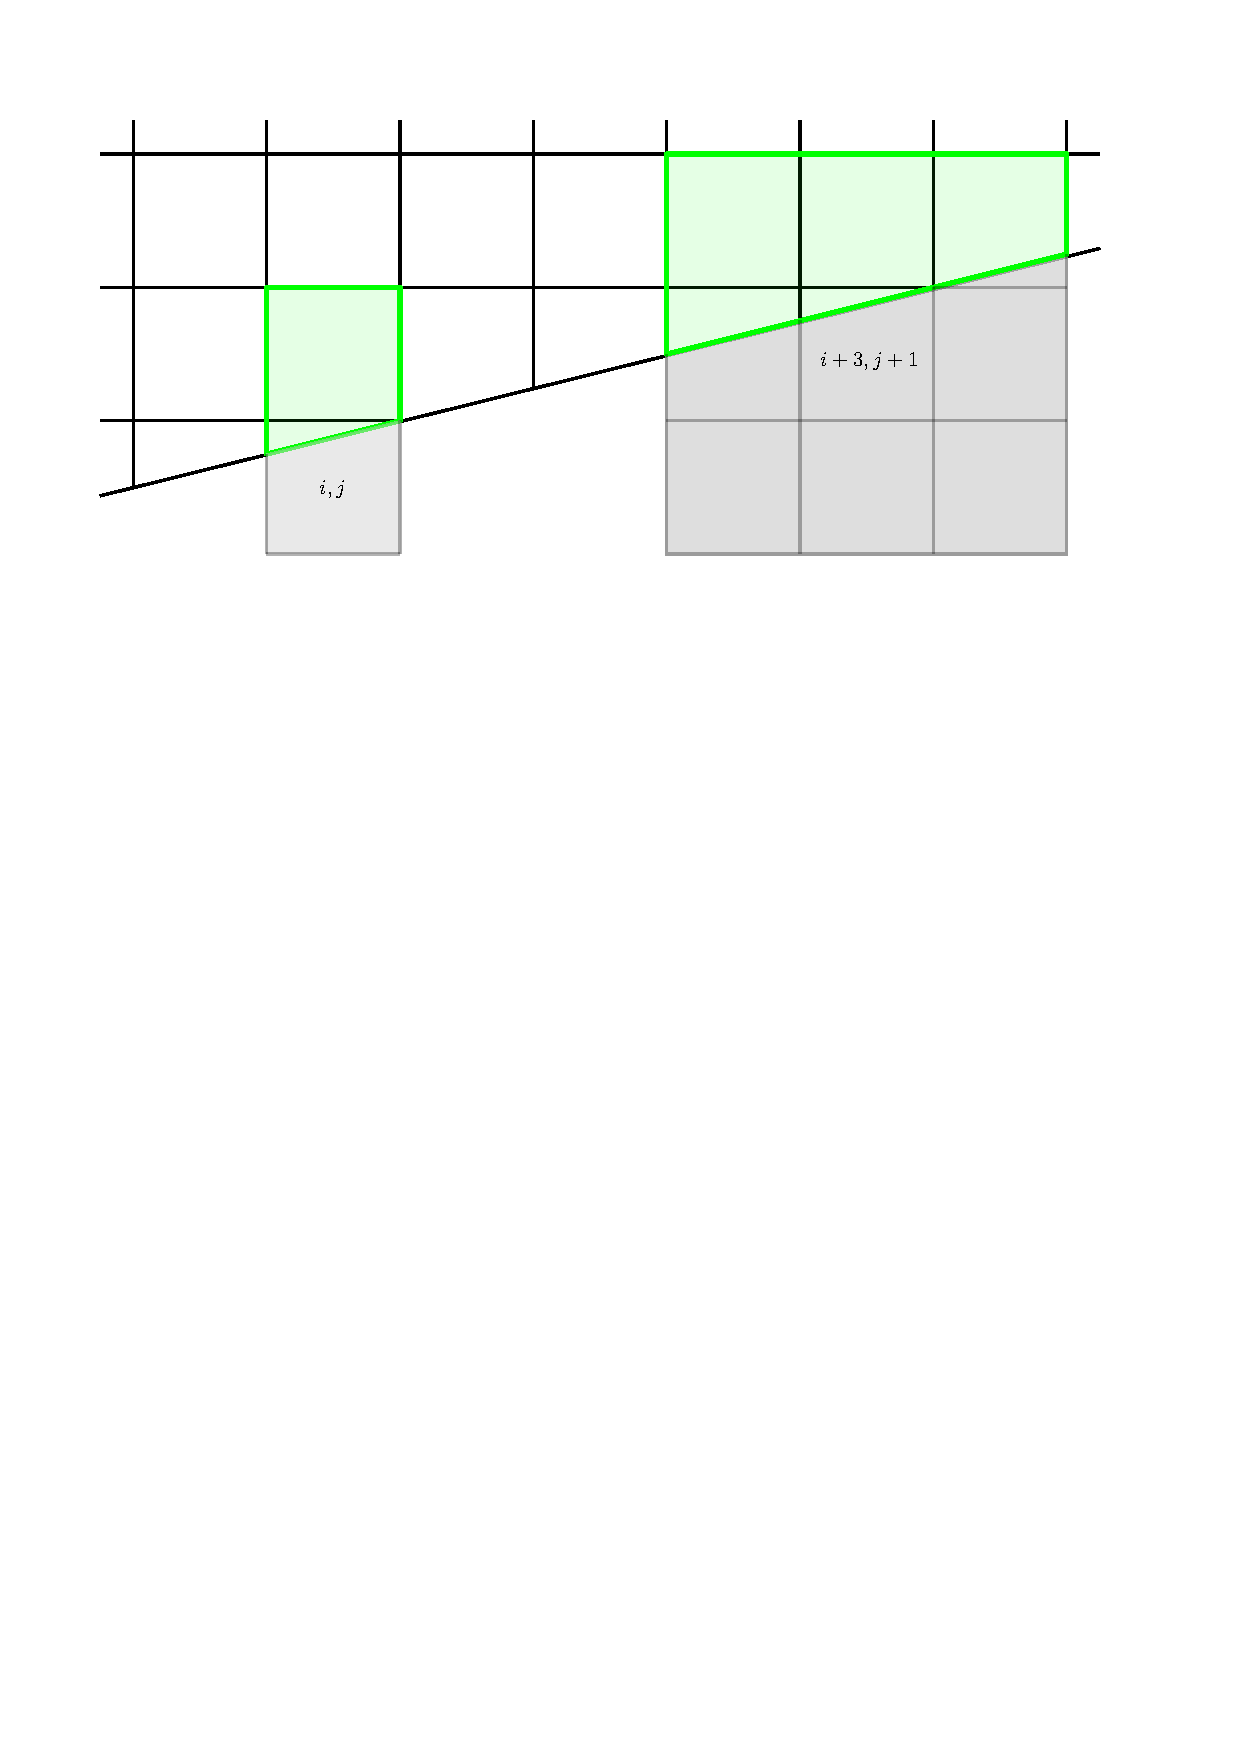
\includegraphics[width=0.5\linewidth]{figs/neighborhoods.pdf}
    \caption{\sf On the left, a small cell is merged with a cell in the direction closest to the 
    	boundary normal.  On the right, a small cell is merged with neighbors that are at most one cell away, i.e., cells located in the $3\times3$ tile centered on $(i+4,j+1)$.}
    \label{fig:neighborhoods}
\end{figure}

The larger the neighborhood the more diffusive the results. Thus we do not want neighborhoods that 
are too large.  However, they must satisfy a size constraint to dampen unstable growth in the numerical 
solution. To this end, we determine neighborhoods, either normal or centered, such that the
volume of the neighborhood is at least half the volume  of an uncut cell, i.e., 
\begin{equation} \label{eqn:vmerge}
\sum_{(r,s) \in M_{i,j}} V_{r,s} \geq \frac{1}{2}\Delta x \Delta y,
\end{equation}
where $M_{i,j}$ denotes the set of cell indices that belong to 
merging neighborhood $(i,j)$.    
In one dimension it has been shown \cite{mjb:stability2} that a cut cell at the boundary 
that is at least half the regular cell size  is stable using a full time step $\Delta t$.  
We have not encountered any issues with this choice in two dimensions.

For smooth solutions a centered neighborhood is sufficient, but for shocks this yields unsatisfactory results. Therefore, we use the normal neighborhood everywhere possible.
The normal neighborhood cannot be used when, e.g., a neighboring cell is also cut and the
merging neighborhood is not sufficiently large (Figure \ref{fig:normalneighborhood}).  In this case, we must use central merging with cells on a $3\times3$ tile (Figure \ref{fig:3x3neighborhood}), or, if that merging neighborhood is not large enough, with cells on the $5 \times 5$ tile.
In this Figure, the gray cells are exterior to the fluid domain, and
are drawn for context.



After forming the merging neighborhoods, each cell counts the number of neighborhoods it belongs to.
For cell $(i,j)$, this neighborhood count is called $N_{i,j}$.

\begin{figure}[h]
\hspace*{.5in}
	\subfloat[\sf Normal neighborhood (in red) for the cut cell $(i,j)$.]{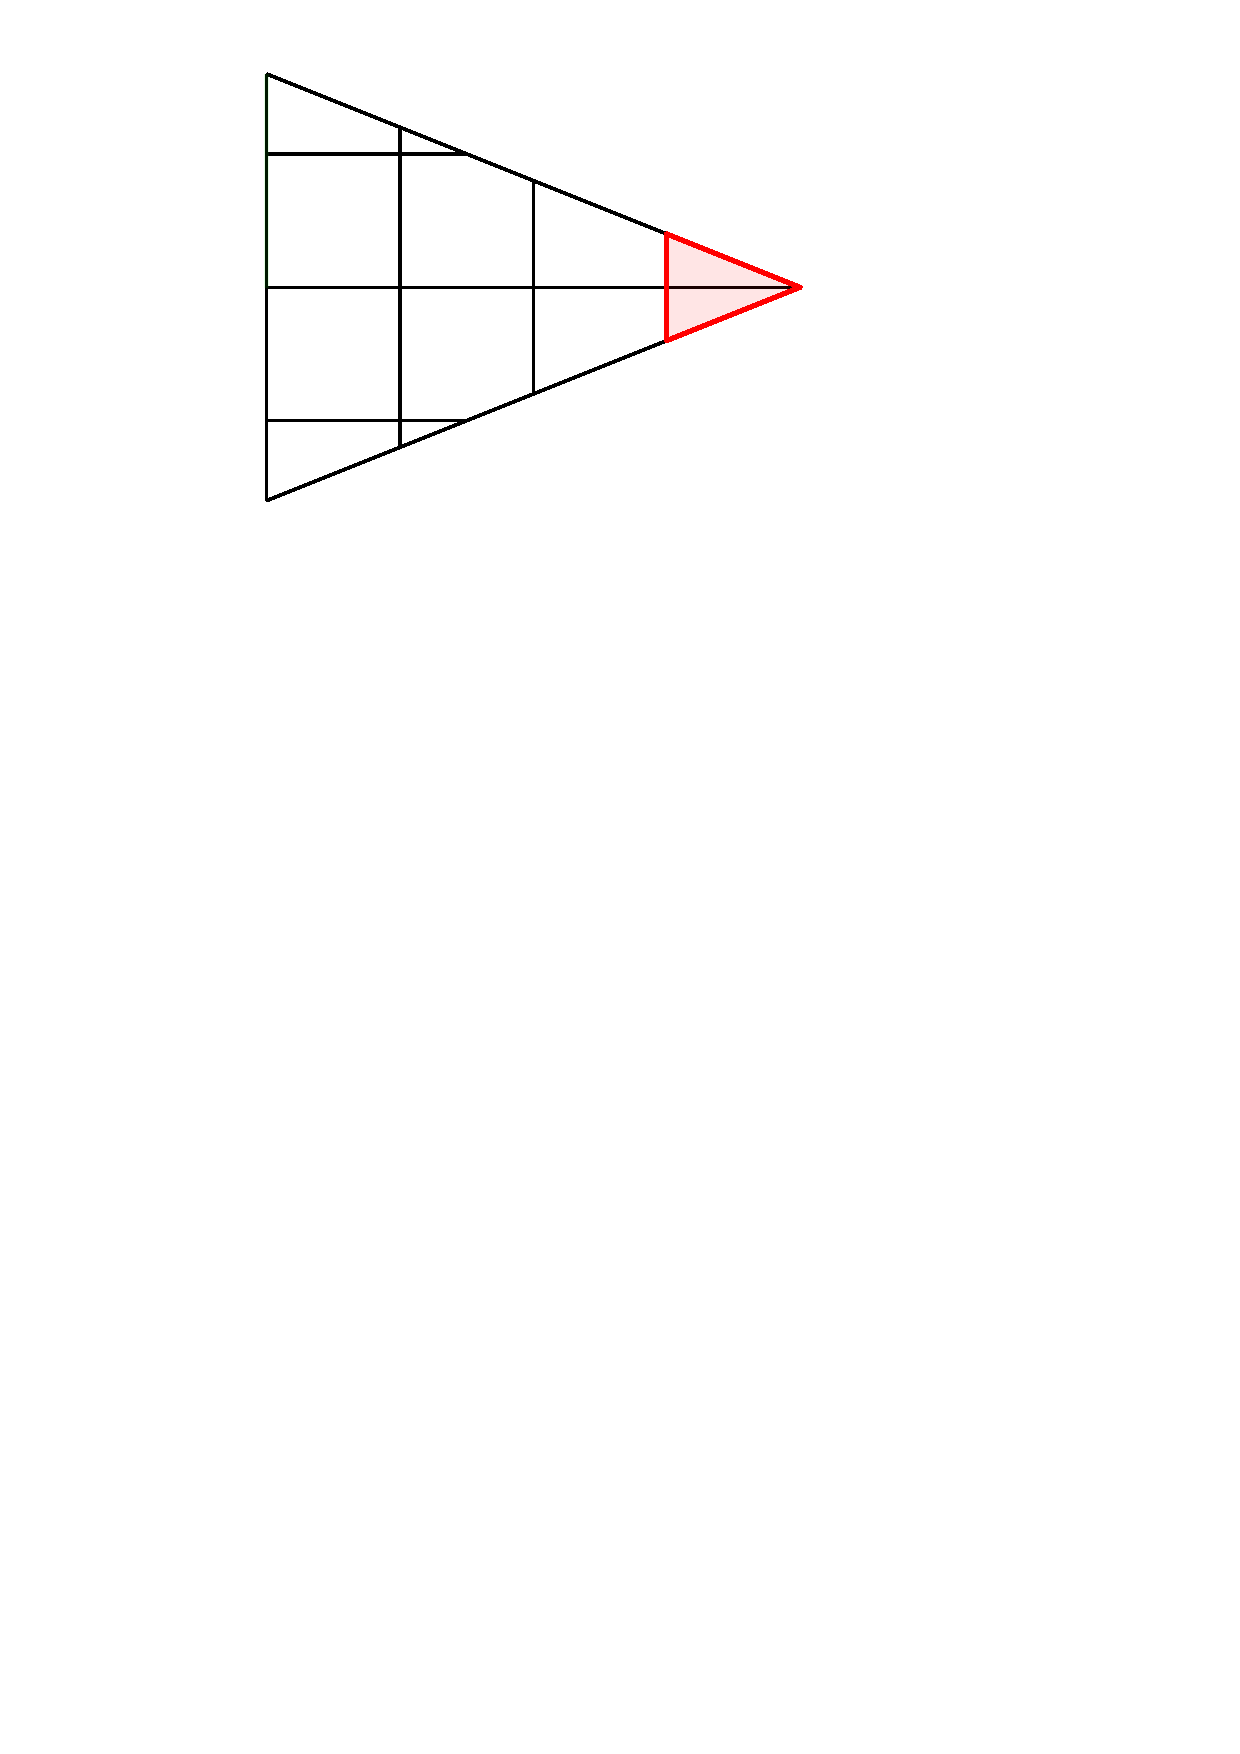
\includegraphics[width=.30\textwidth]{figs/normaldirection1.pdf} \label{fig:normalneighborhood}}
	\hfill
	\subfloat[\sf $3\times 3$ merging neighborhood (in green) for centered on cut cell $(i,j)$.]{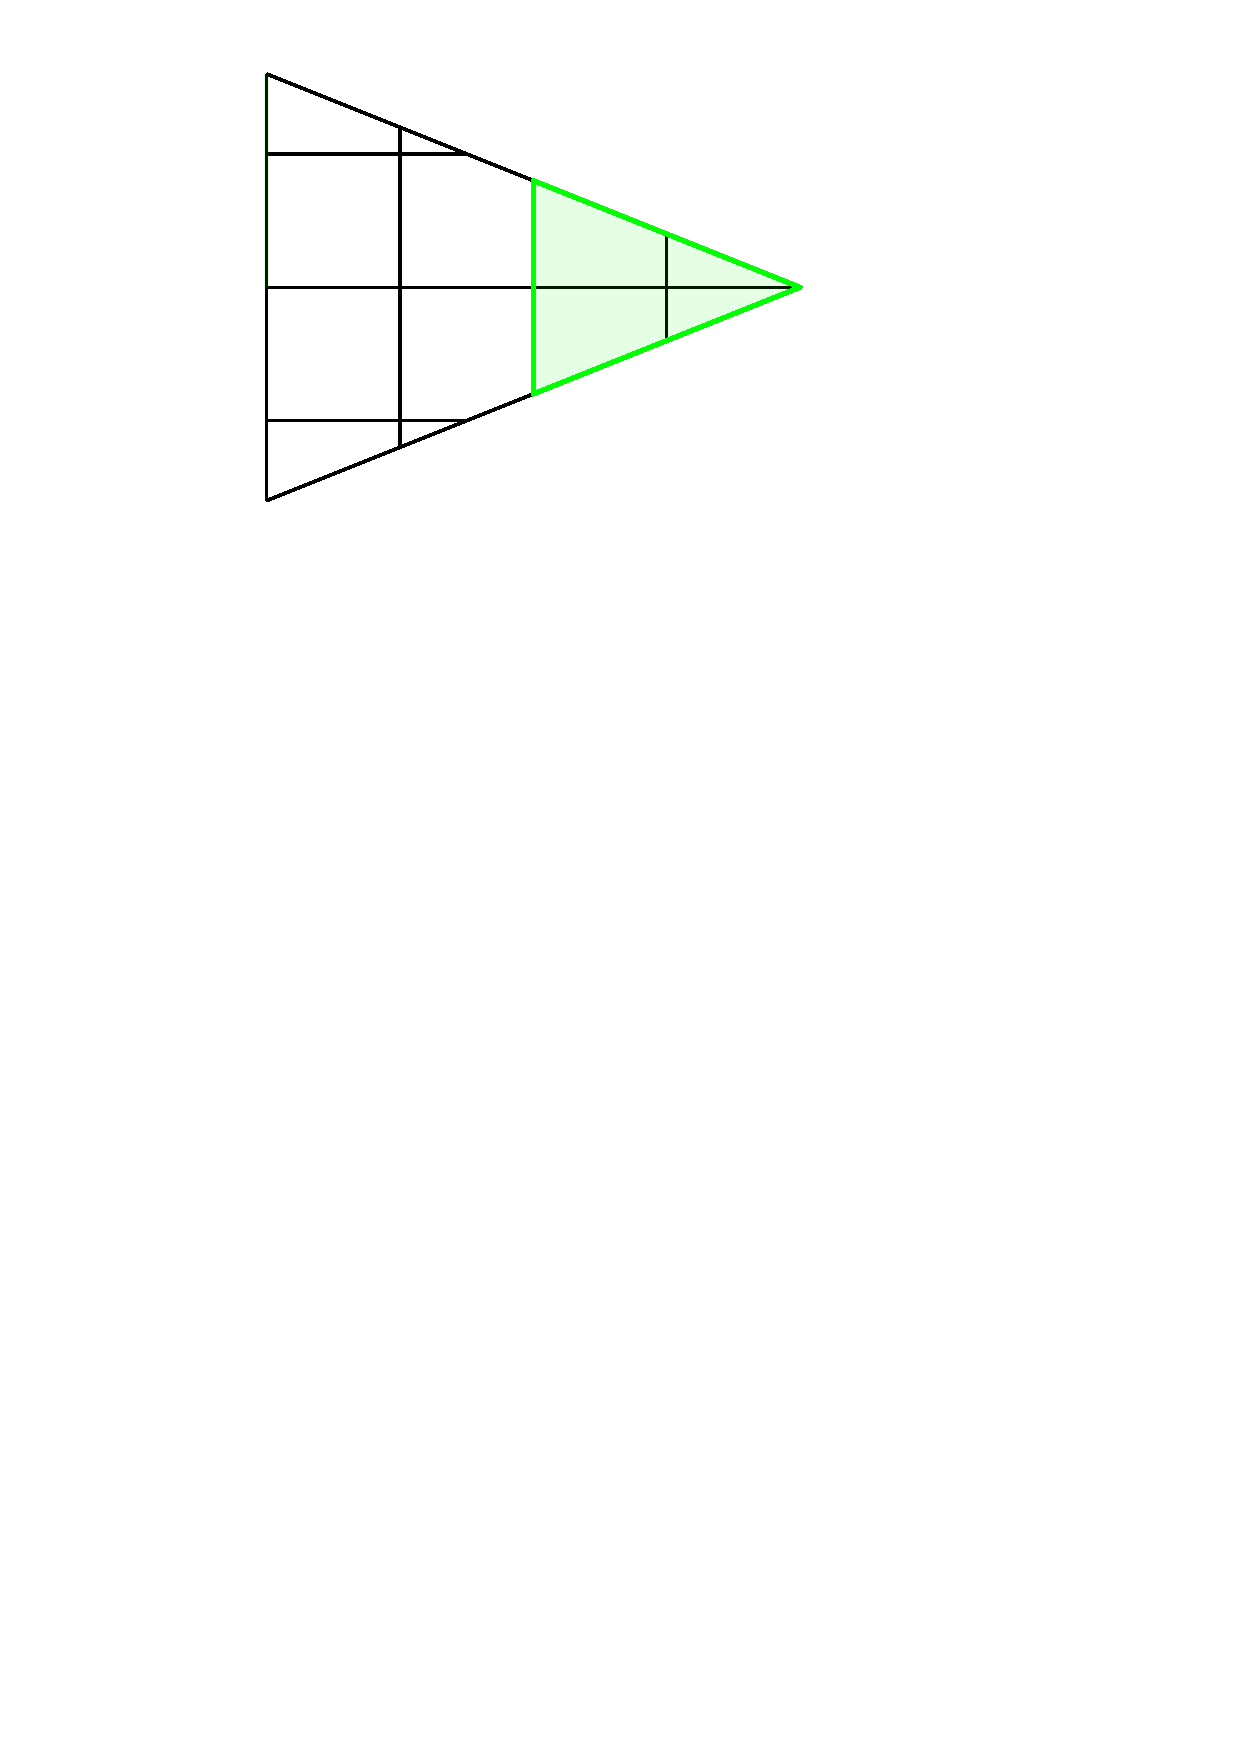
\includegraphics[width=.35\textwidth]{figs/normaldirection2.pdf} \label{fig:3x3neighborhood}}
	\caption{\sf It can happen that merging only in the normal neighborhood is not 
        large enough, e.g. if the small cell merges with another small cell, and \eqref{eqn:vmerge} is not satisfied.  In this case, we use the $3\times 3$ neighborhood. }
\end{figure}


To more clearly illustrate overlapping merging neighborhoods in two dimensions, consider the cut cell 
mesh in Figure \ref{fig:2nborTile}.   The neighborhoods $(i,j)$ and $(i,j+1)$ overlap on cell $(i,j+1)$ in 
the base grid.  The normal merging neighborhood of cut cell $(i,j)$ is highlighted in green in Figure \ref{fig:2nborTile1}.  
Since cell $(i,j)$ does not satisfy the volume constraint in \eqref{eqn:vmerge},
the neighborhood of $(i,j)$, $M_{i,j}$, must include both $(i,j)$ and $(i,j+1)$.  
The neighborhood associated with $(i,j+1)$ in highlighted in green in Figure \ref{fig:2nborTile2}.  
Since the volume of cell $(i,j+1)$ satisfies the volume constraint in \eqref{eqn:vmerge}, $M_{i,j+1}$, only contains cell $(i,j+1)$.
  
\begin{figure}[h]
	\centering
	\subfloat[Merging neighborhood of cell $(i,j)$.]{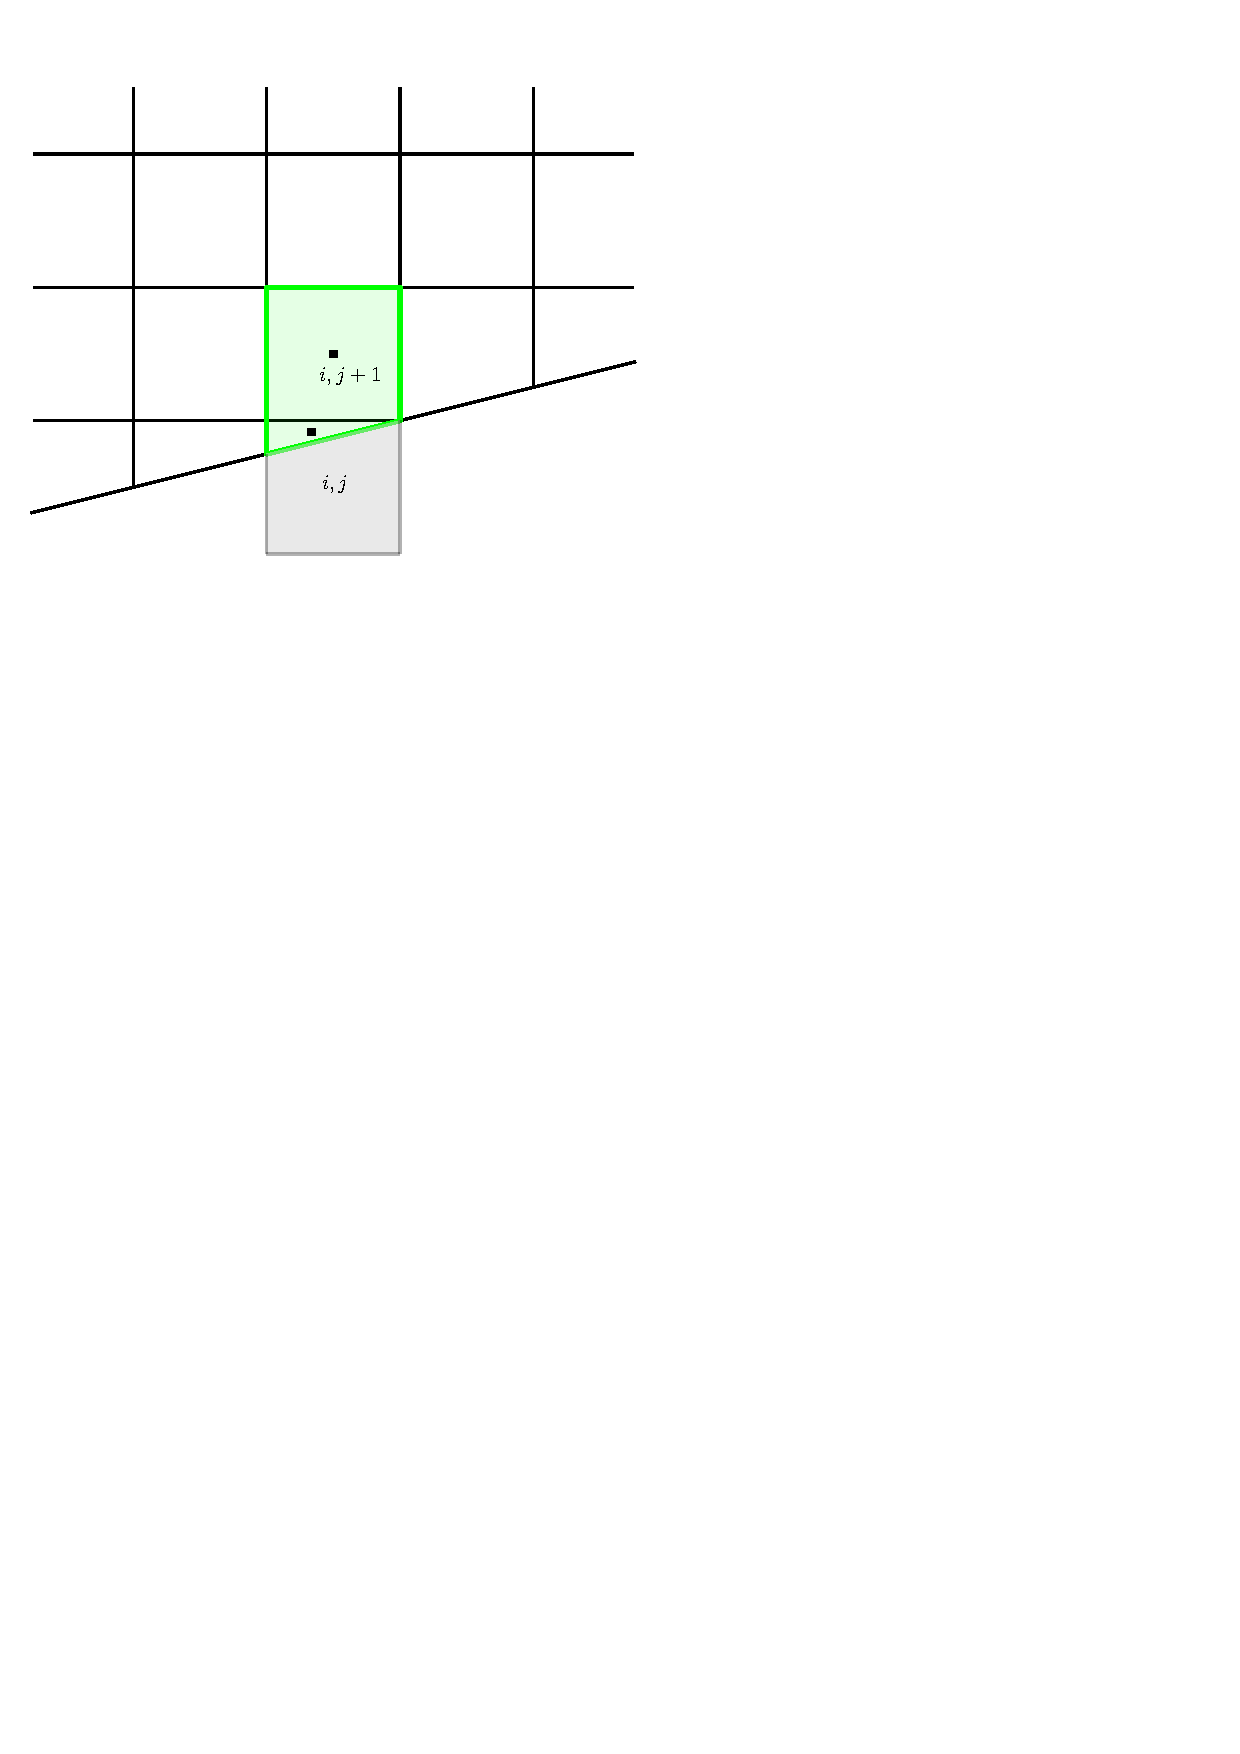
\includegraphics[width=0.30\textwidth]{figs/modelexample2D_2.pdf} \label{fig:2nborTile1}}
	\qquad
	\subfloat[Merging neighborhood of cell $(i,j+1)$.]{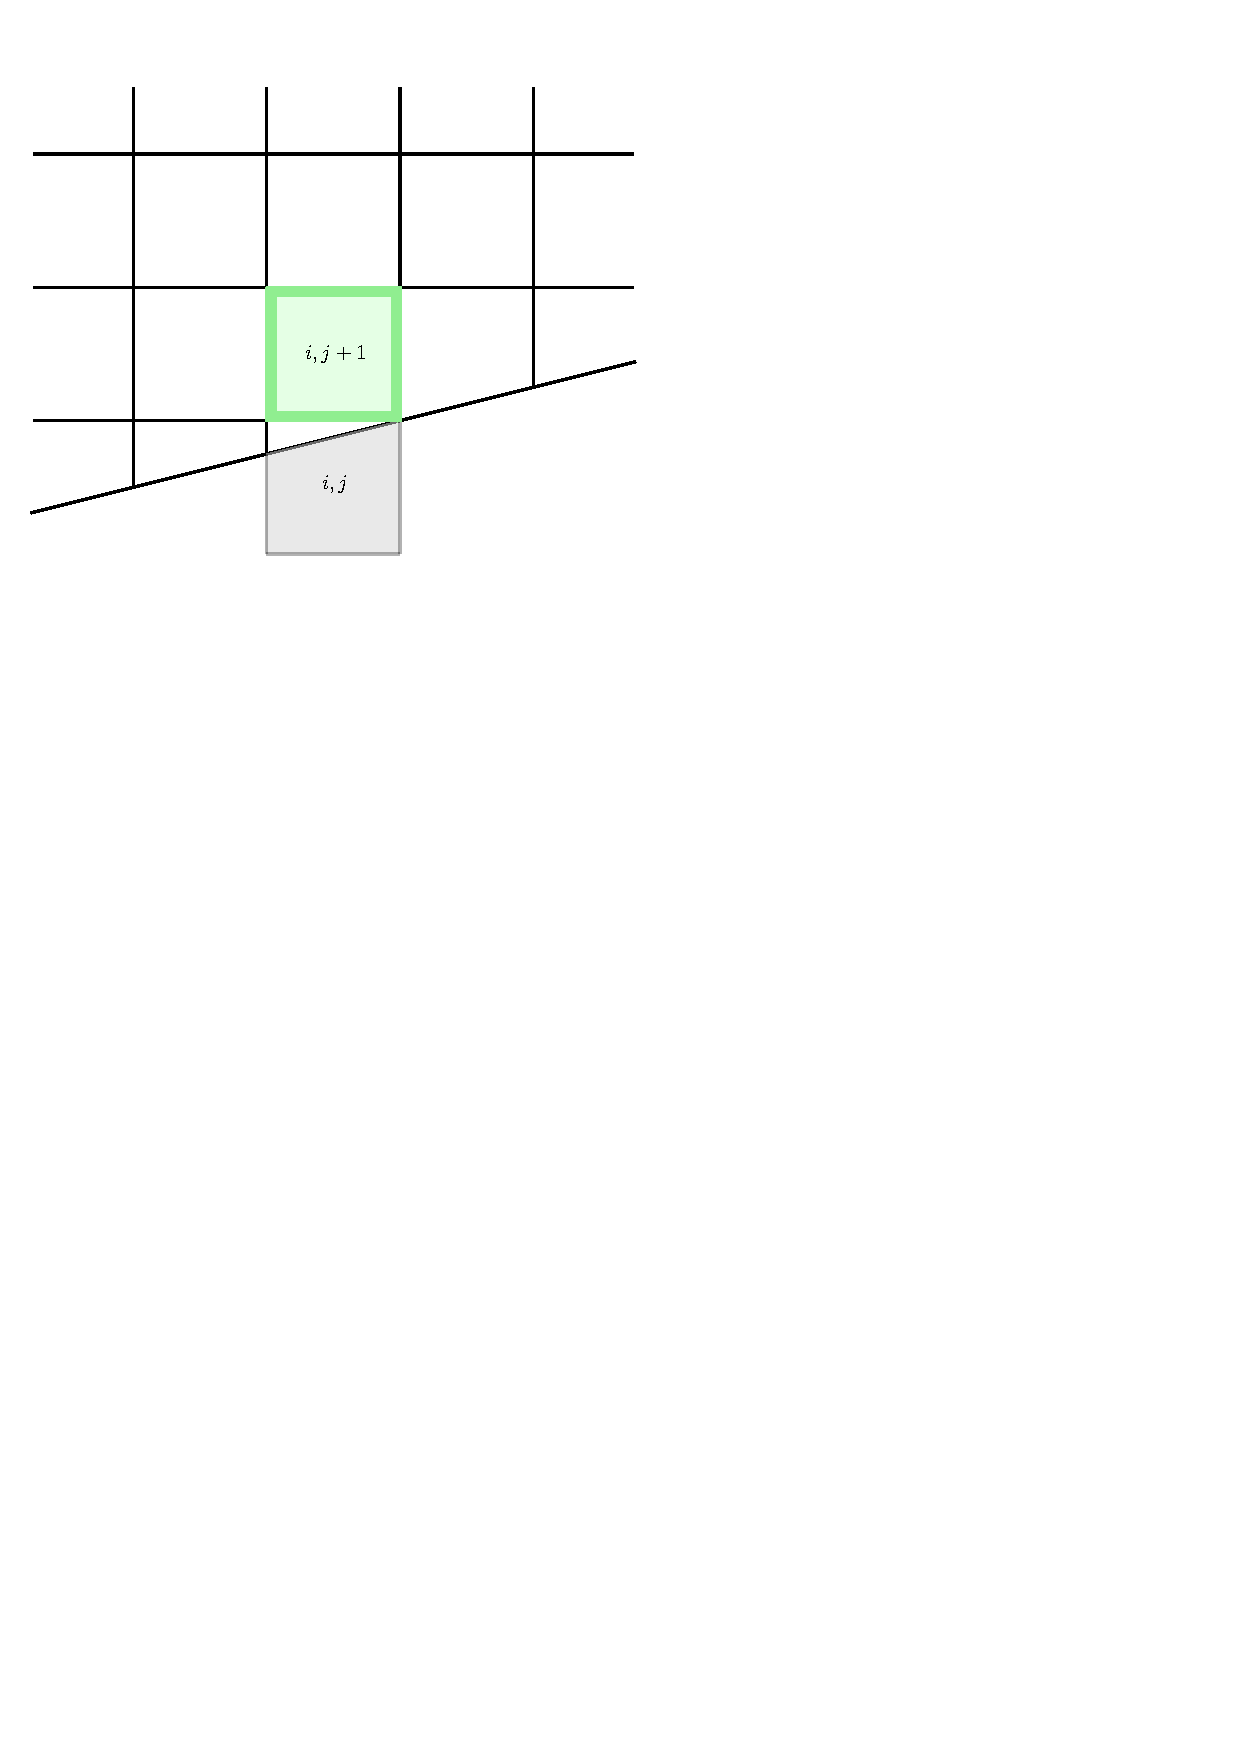
\includegraphics[width=.30\textwidth]{figs/modelexample2D_1.pdf} \label{fig:2nborTile2}}
	\caption{\sf Example of two neighborhoods, highlighted in green, that overlap on cell $(i,j+1)$.} \label{fig:2nborTile}
\end{figure}

% If the neighboring cell 
% is also cut, it can happen that the
% merged cell is not sufficiently large (SHOW EXAMPLE?). 
% Next we try a 2 by 2
% neighborhood, including the original cut cell. Later we also show
% results using a 3 by 3 neighborhoods. However the larger the
% neighborhood the more diffusive the results.

% Note that this does not have the difficulty of cell merging, since 
% overlapping neighborhoods are allowed. 

%\item
%{\bf Each cell counts how many neighborhoods it is a part of.}

%\vspace*{.1in}
%\subsubsection*{Overlap count}
%We compute $N_k$, the number of neighborhoods cell $k$ is part of.
%A full cell is its own merging neighborhood, since it has sufficient
%volume all by itself.
%However, we will still refer to all cells as having a
%merging neighborhood.  
%Figure \ref{fig:overlappingneighs} shows an example of a
%cut cell mesh with all merging neighborhoods plotted.  Also displayed
%are the number of overlapping neighborhoods for each cell. 
%This is what we call the neighborhood {\em count} referred to above.
%\begin{figure}
%	\subfloat[]{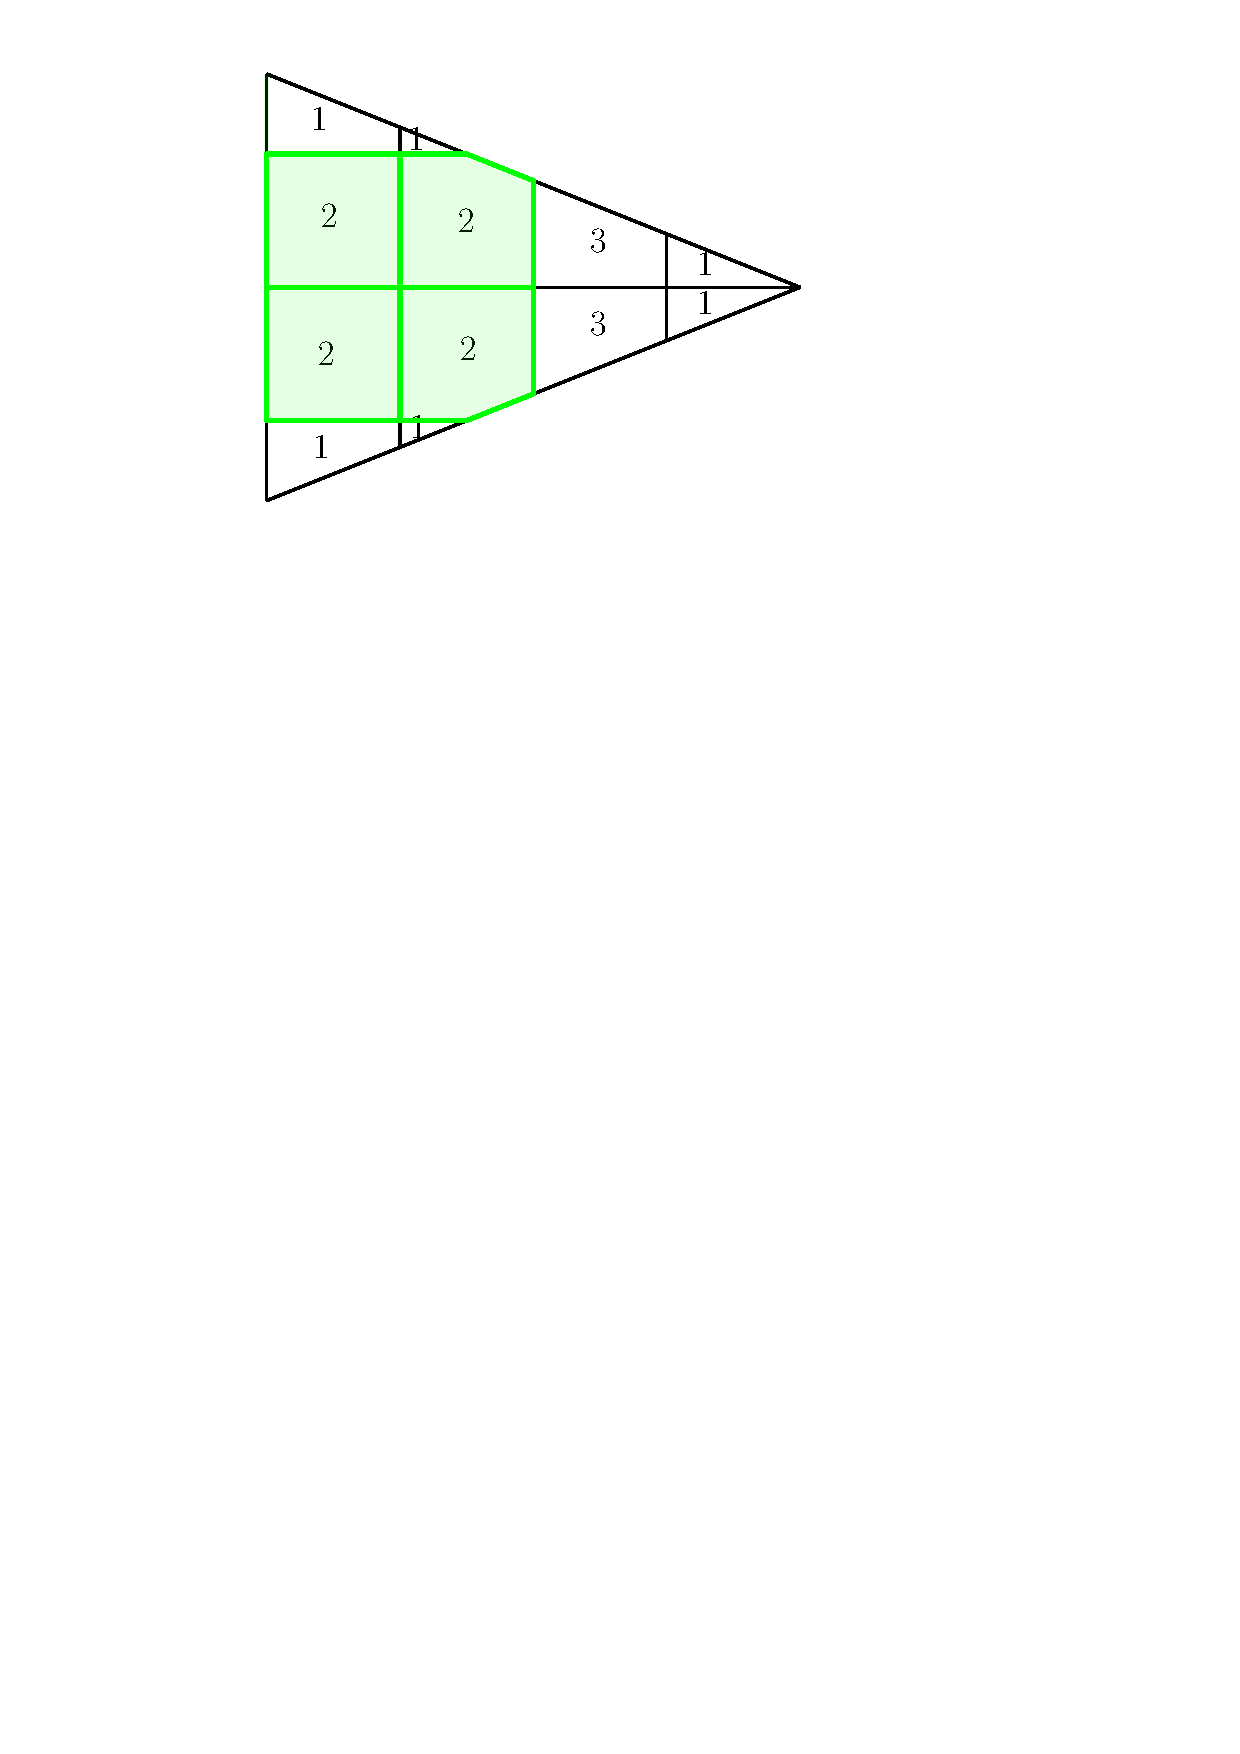
\includegraphics[width=.24\textwidth]{figs/numoverlaps1.pdf} \label{fig:numoverlaps1}}
%	\hfill
%	\subfloat[]{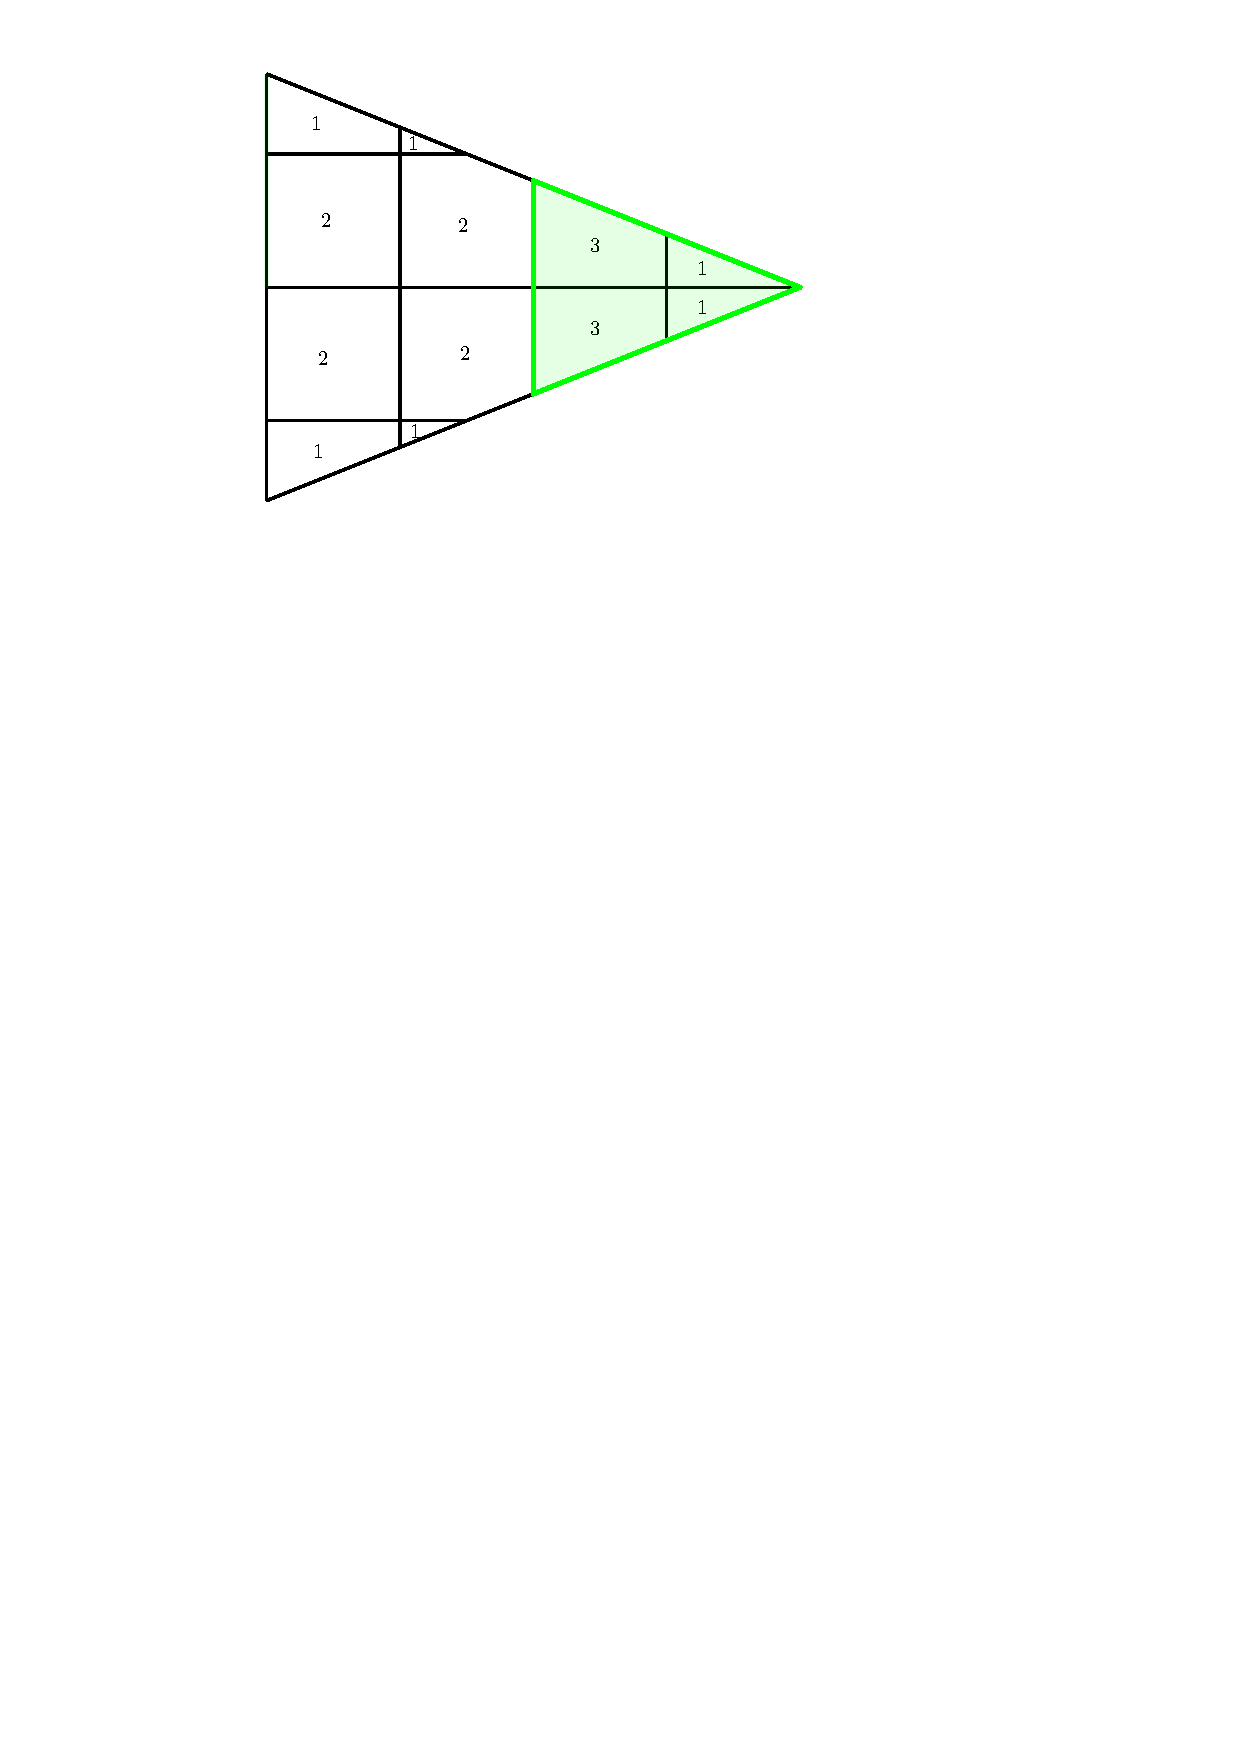
\includegraphics[width=.24\textwidth]{figs/numoverlaps5.pdf} \label{fig:numoverlaps4}}
%	\hfill
%	\subfloat[]{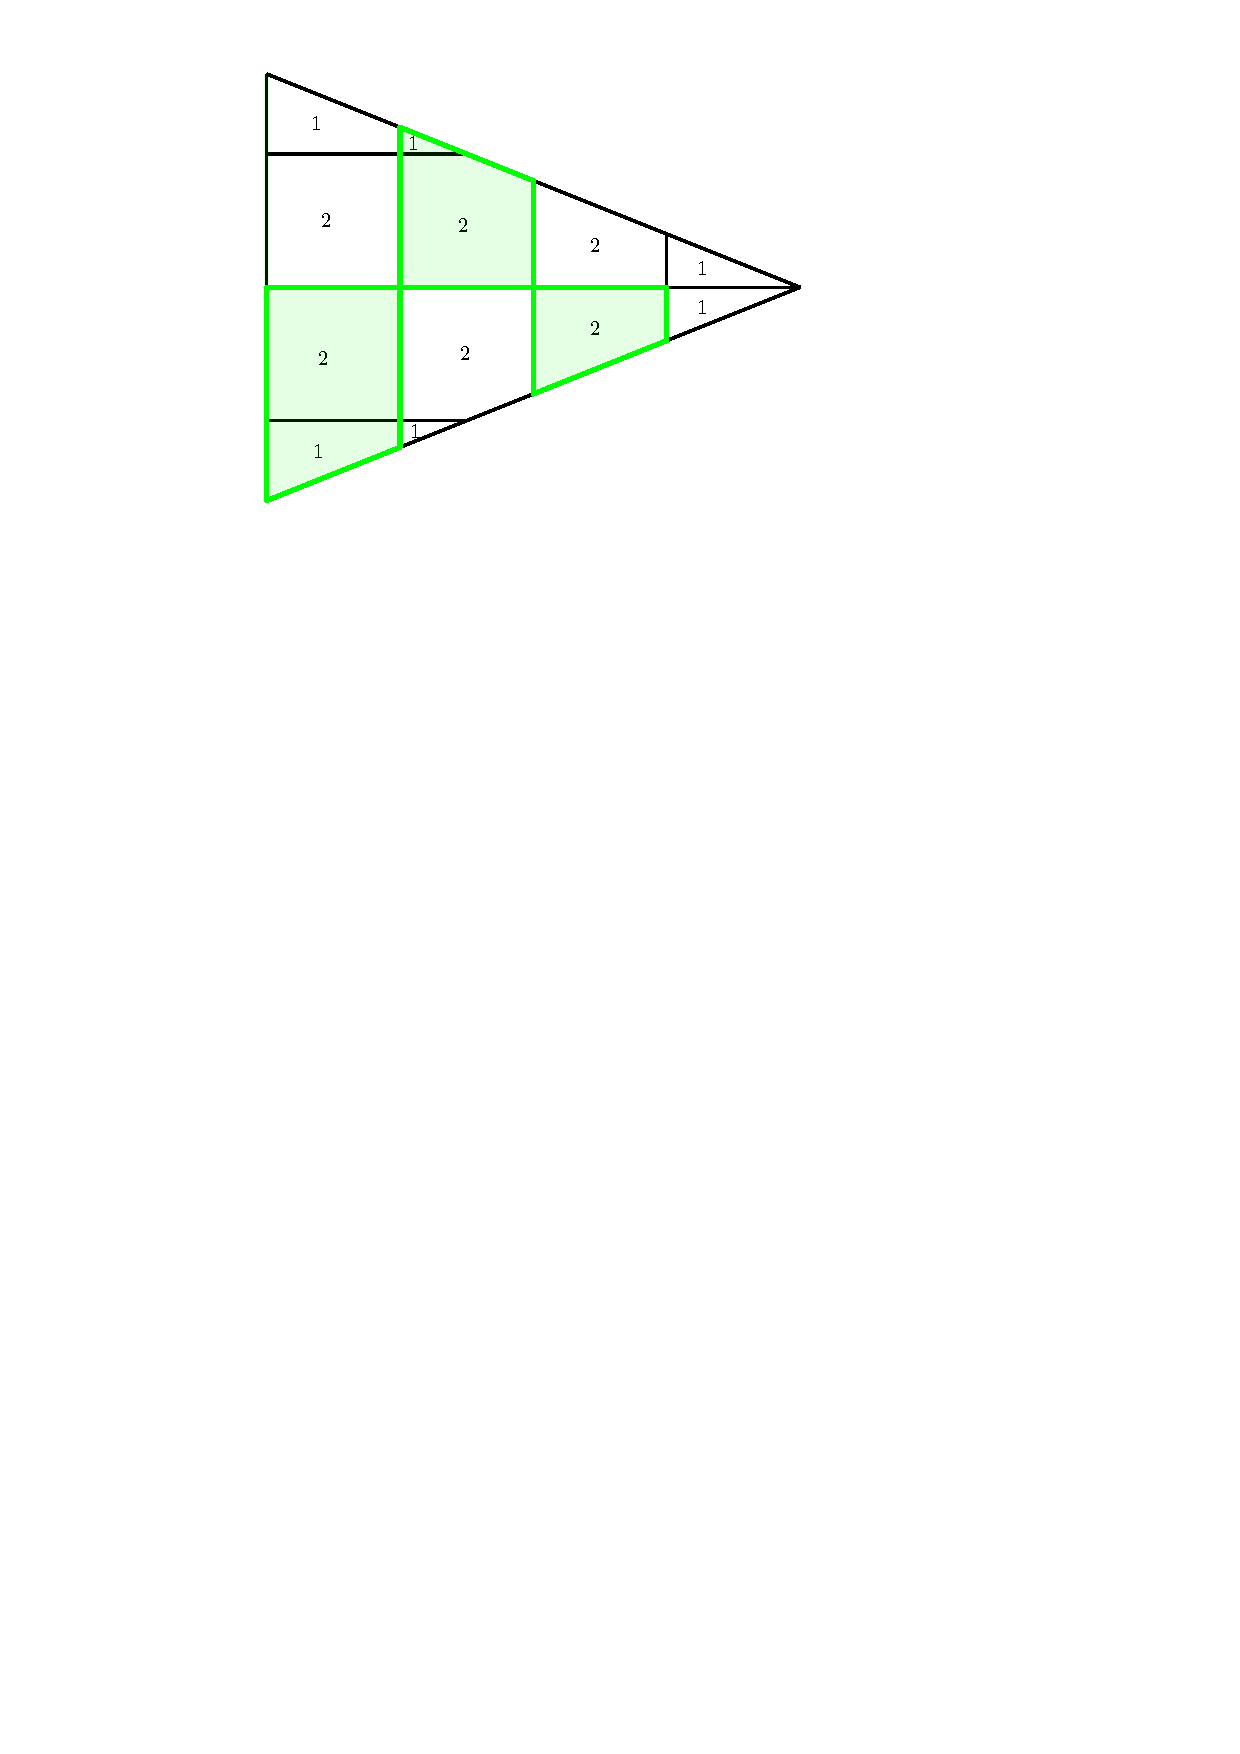
\includegraphics[width=.24\textwidth]{figs/numoverlaps2.pdf} \label{fig:numoverlaps2}}
%    \hfill
%	\subfloat[]{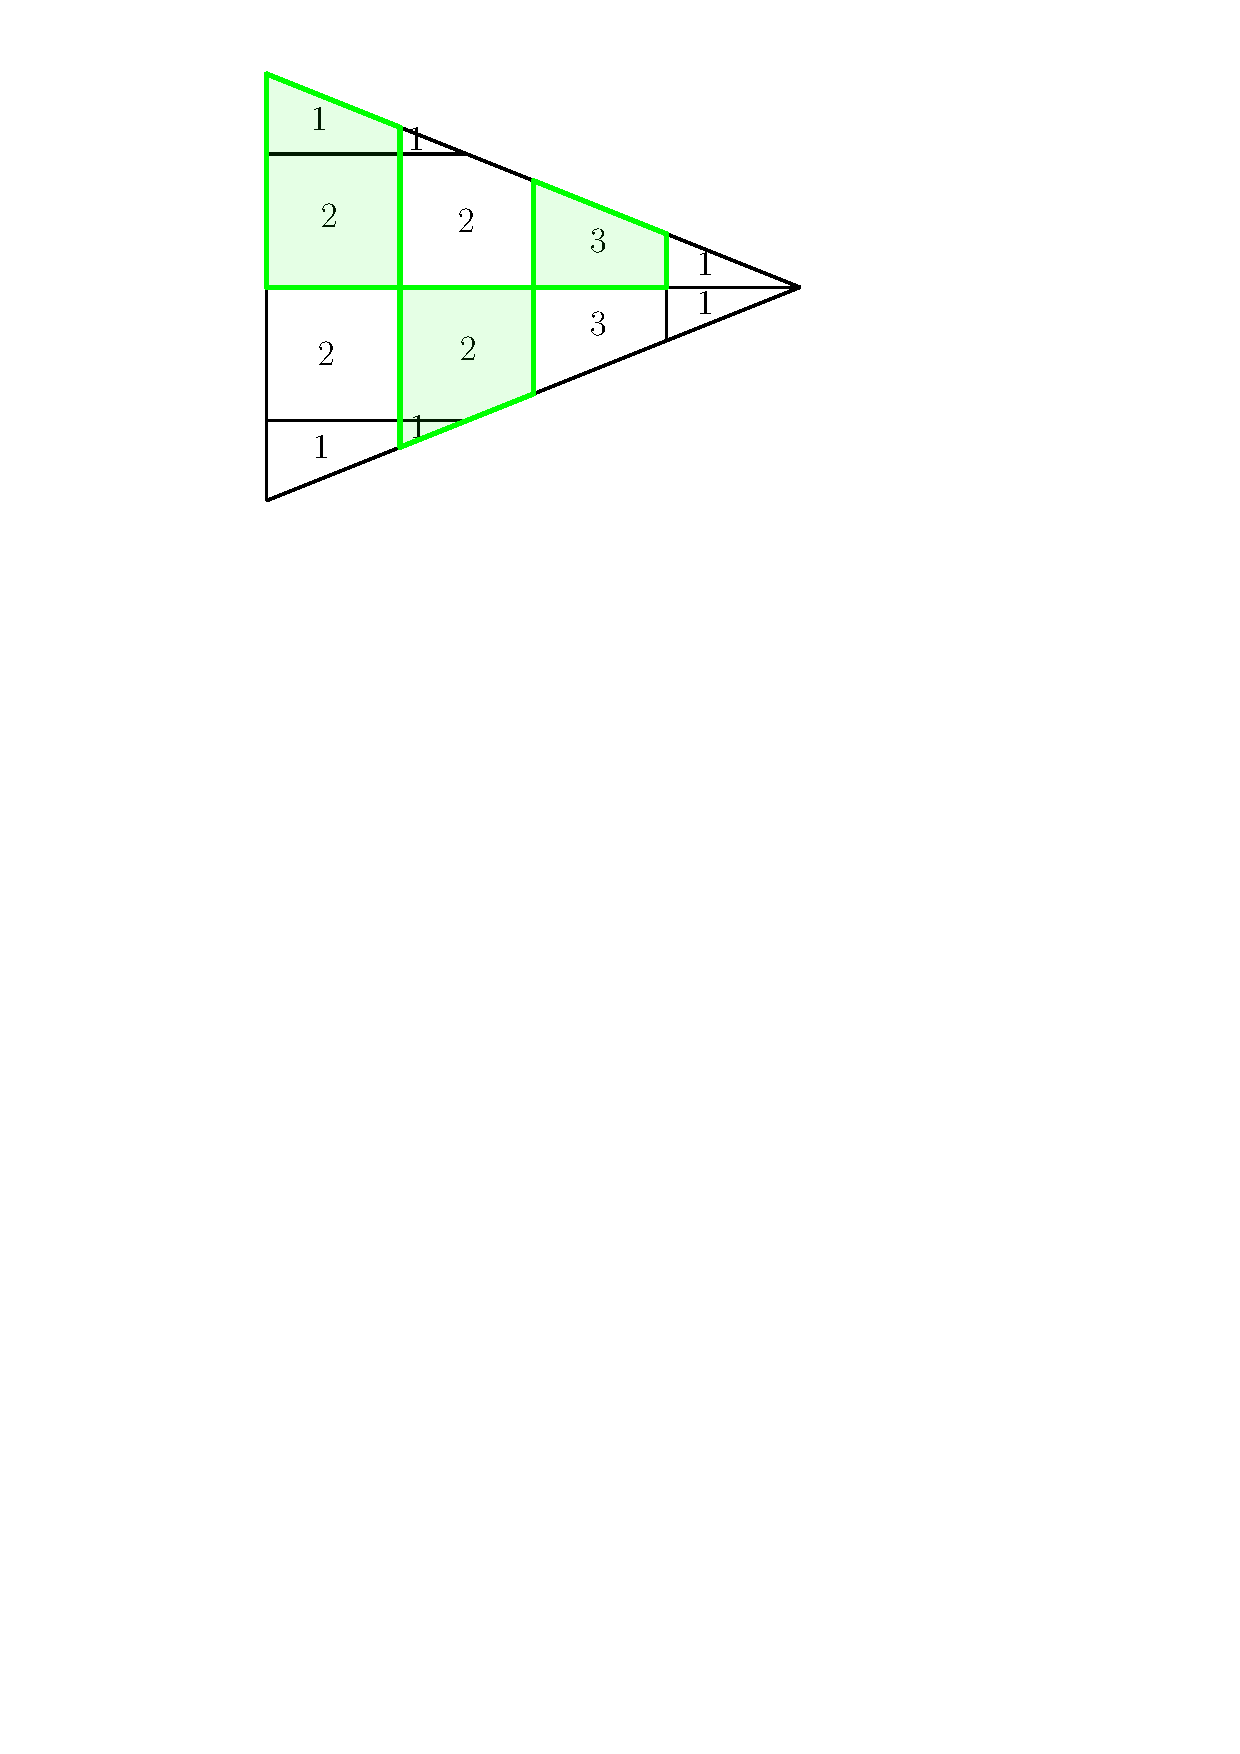
\includegraphics[width=.24\textwidth]{figs/numoverlaps3.pdf} \label{fig:numoverlaps3}}
%	\caption{\sf All merging neighborhoods on an example cut cell mesh (in green).  We display the number of overlapping merging neighborhoods on each cell. Note, in figure \ref{fig:numoverlaps4}, there are two merging neighborhoods that occupy the same location, one per small cell in the right corner.} \label{fig:overlappingneighs}
%\end{figure}
%But a full cell can be part of 
%two (or more)  merging neighborhoods  if it is placed next to 
%one (or more)  tiny cut cells. This is the case for the highlighted green
%cell on the left in figure
%\ref{fig:neighborhoods}. The full cell is its own merging neighborhood, 
%as well as being part of the cut cell's neighborhood. Thus the full cell has a
%count of 2, and the cut cell has a count of 1.
%
%Most full
%cells are only members of their own tile and will have a count of one.
%Only cells within a narrow band of the cut cells will have a count
%larger than one.

%\item
%{\bf Each neighborhood computes its weighted centroid and volume.}

\subsubsection*{Weighted centroids and volumes}

The neighborhood's weighted volume is defined as
\begin{equation}
\label{eqn:voldef}
{\widehat V}_{i,j} =  \sum_{(r,s) \in M_{i,j} } \,  \frac{V_{r,s}}{N_{r,s}}.
\end{equation}
where $M_{i,j}$ is the set of cells in the neighborhoods associated with cell $(i,j)$. 
The weighted centroid of the merging neighborhood is defined as
\begin{equation}
\label{eqn:centroiddef}
({\widehat x}_{i,j},{\widehat y}_{i,j}) = \frac{1}{\widehat V_{i,j}} \sum_{(r,s) \in M_{i,j} } \,  \frac{V_{r,s}}{N_{r,s}}(x_{r,s},y_{r,s}),
\end{equation}

In general, the weighted volume is not the physical volume of 
the merging neighborhood 
unless the neighborhood  is not overlapped by any other neighborhoods 
(for example, cells $-3$ and $3$ in Figure 2).  Similarly, the weighted and physical 
centroids are different unless the overlap count on each cell in the neighborhood is the 
same, $N_{r,s} = N_{p,q} ~ \forall (r,s), (p,q) \in M_{i,j} $.  
This is because the overlap counts in \eqref{eqn:centroiddef} would cancel, leading to identical  weighted and physical 
centroids of the neighborhood.


%\begin{figure}[h]
%    \centering
%    \hspace*{.5in}
%    \subfloat[]{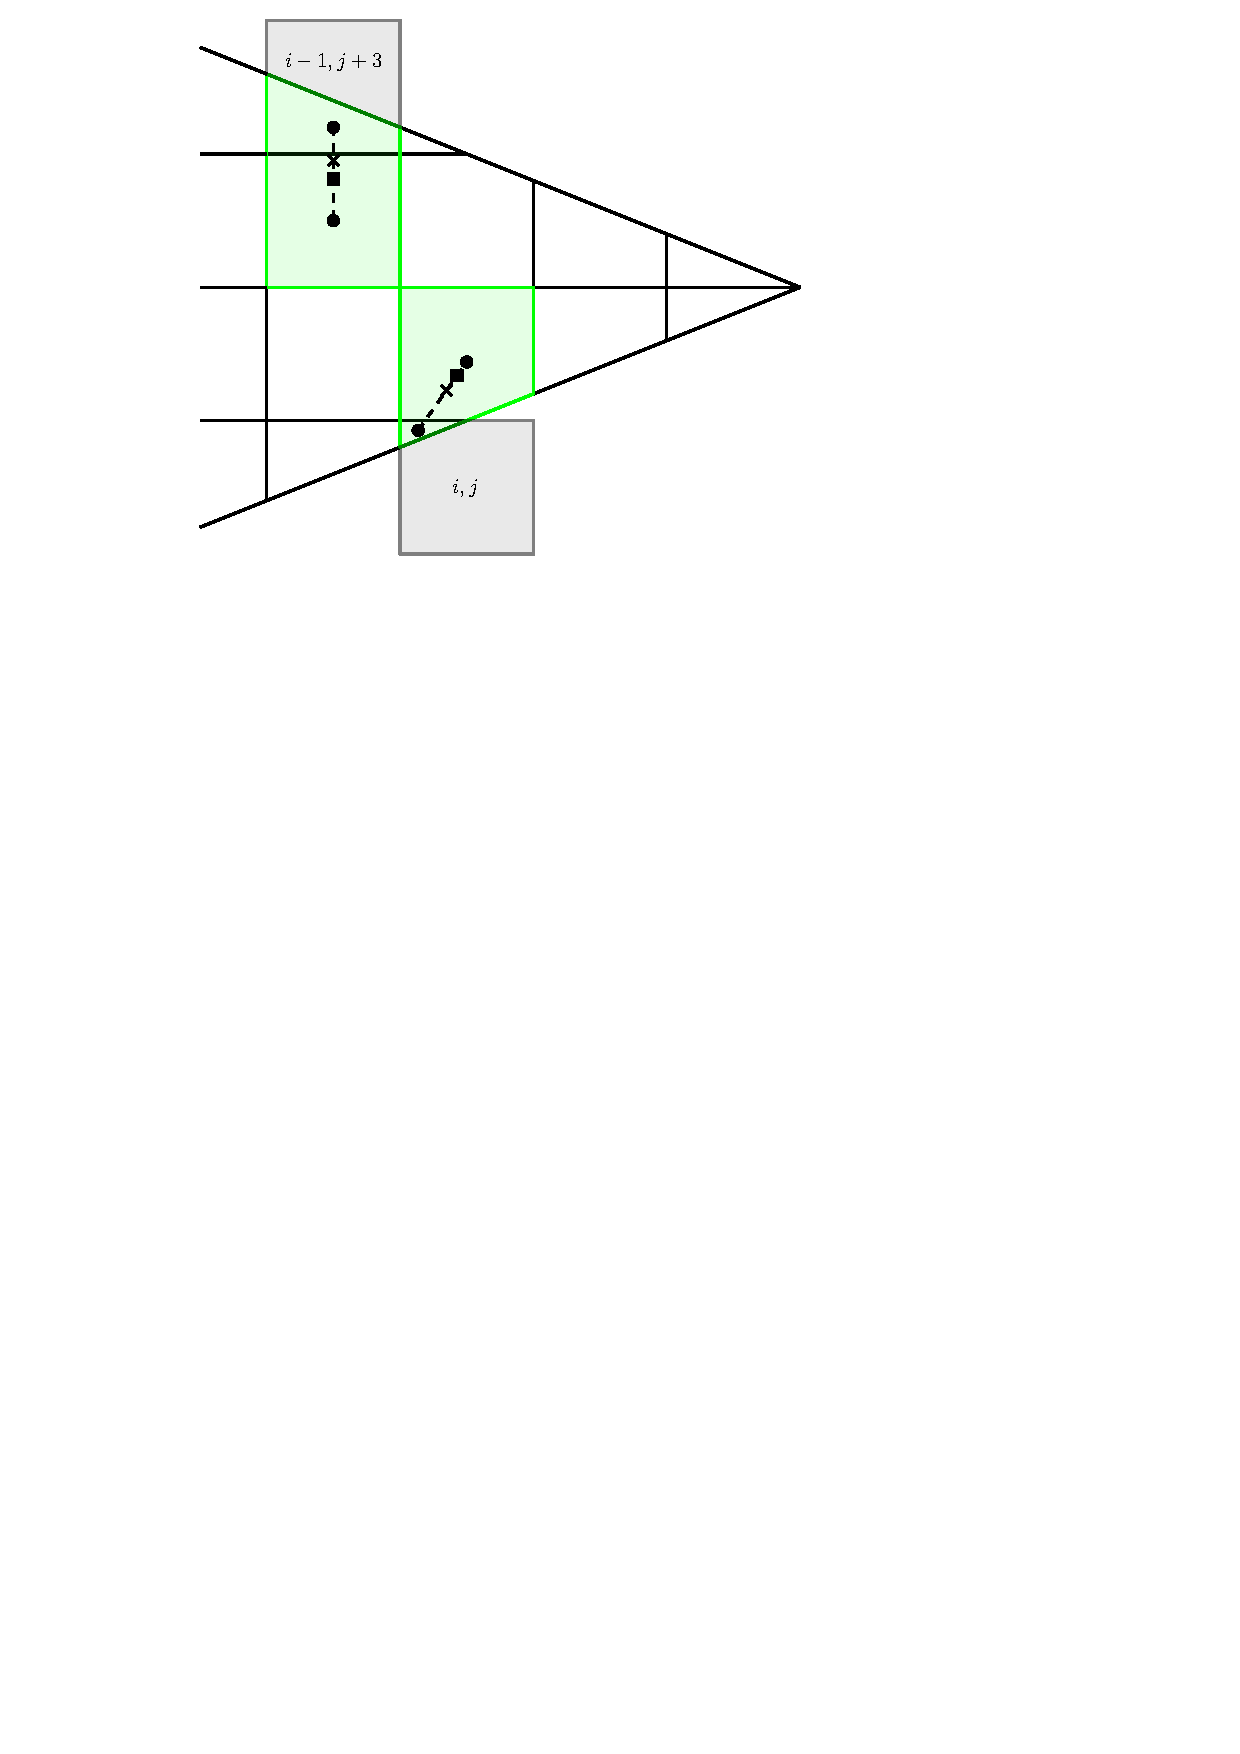
\includegraphics[width=0.4\linewidth]{figs/centroids3.pdf}}
%%    \subfloat[]{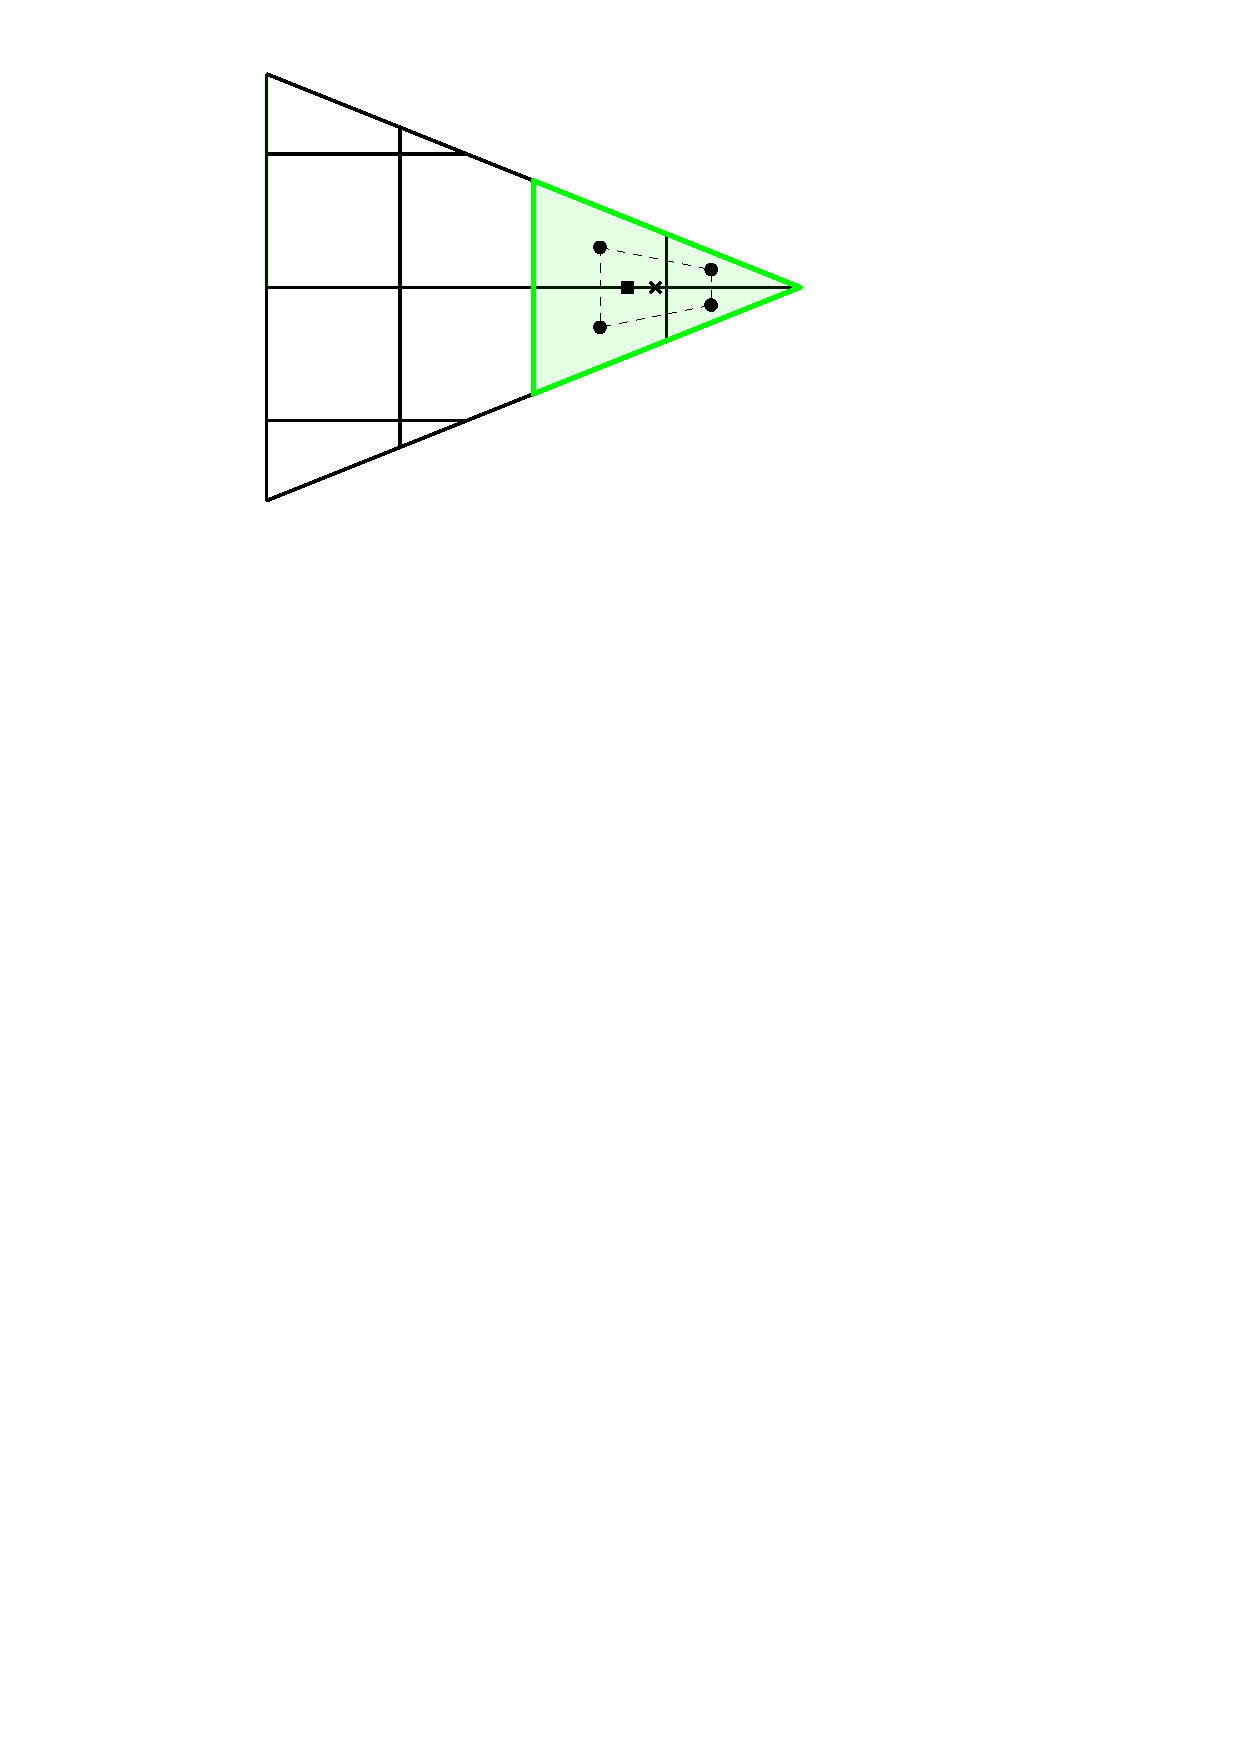
\includegraphics[width=0.35\linewidth]{figs/centroids4.pdf}}
%    \caption{\sf The physical and weighted centroids of the merging neighborhoods associated to cells $(i,j)$ and $(i-1, j+3)$ are indicated with a square ($\blacksquare$) and a cross ($\times$), respectively. The centroids of the Cartesian and cut cells are indicated with a solid circle ($\bullet$).  Note that the physical centroids and weighted centroid of the cut cell neighborhoods do not necessarily coincide.}
%    \label{fig:centroids}
%\end{figure}

%\end{itemize}

% \begin{figure}[h!]
% \begin{center}
% 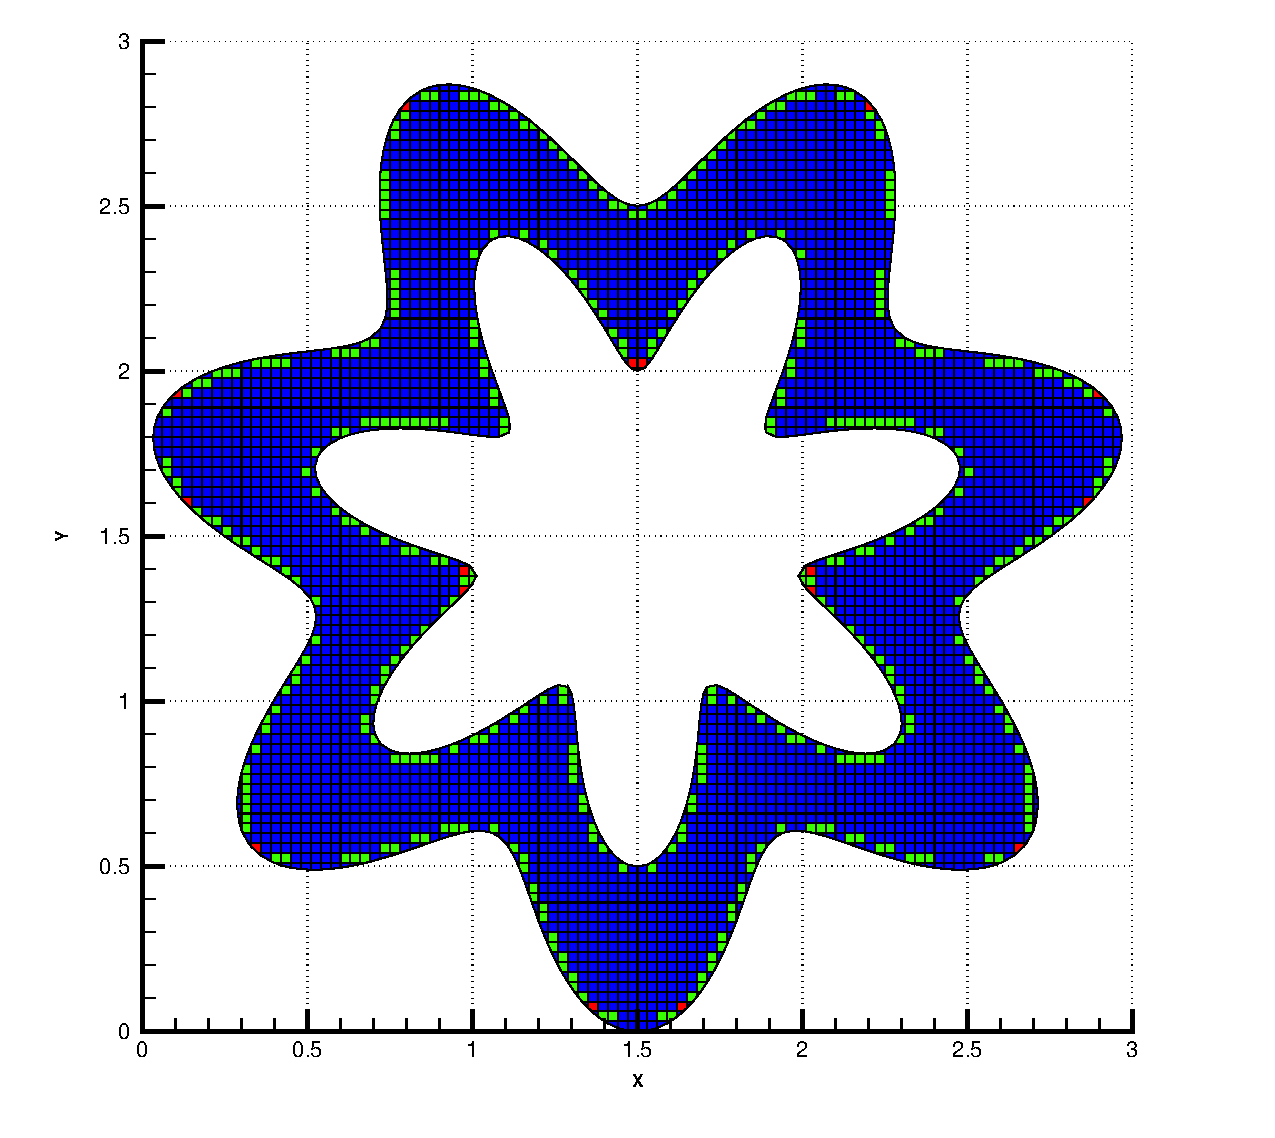
\includegraphics[width=4.5in]{figs/waveynumhoods.eps}
% \caption{\sf Domain from example XX.  Figure shows how many
% neighborhoods each cell belongs to: 
% one (white), two (blue), or three (red).
% The full example is shown in section \ref{sec:compResults}.}
% \label{fig:2nborTile}
% \end{center}
% \end{figure}



%\vspace*{.1in}
\subsection{State redistribution postprocessing} \label{sec:srd_postprocessing}


In this section, we describe postprocessing on two-dimensional meshes with overlapping neighborhoods.
This is the analogue of postprocessing on one dimensional nonuniform grids in Section \ref{sec:srd1d}.
The SRD stabilization is applied after each stage for the method of lines (Section \ref{sec:mol}) 
or time step for the MUSCL scheme (Section \ref{sec:muscl}), denoted generically as
\begin{equation} \label{eq:stage_step}
\widehat{U} = U^n + \Delta t  L(U^n).
\end{equation}
%where $L$ is the operator in \eqref{eq:molscheme} or from the MUSCL scheme. 
We refer to
$\widehat{U}$ as the provisionally updated solution.


\subsubsection*{Step 1. Compute weighted solution averages on each neighborhood}   

%\vspace*{.1in}
The solution average on each neighborhood is given by
\begin{equation}
\label{tiledef}
\widehat{Q}_{i,j} =  \frac{1}{{\widehat V}_{i,j}} \, \sum_{(r,s) \in M_{i,j}} \,  
\frac{V_{r,s}}{N_{r,s}}  \widehat{U}_{r,s}
\end{equation}
where the volume ${\widehat V}_{i,j}$ is the weighted neighborhood volume defined in \eqref{eqn:voldef}
and $N_{r,s}$ is the number of neighborhoods  associated with cell $i,j$ defined in 
Section \ref{sec:preprocessing}.  
Analogous to the one dimensional case in Section \ref{sec:srd1d}, the weighted solution 
averages are a convex combination of provisional solution averages on the
neighborhood associated with cell $(i,j)$.  

\subsubsection*{Step 2. Reconstruct and limit a gradient on each neighborhood}

For second order accuracy in space we need to compute a gradient on each 
neighborhood, again  using a least squares procedure.
The set of merging neighborhood indices for reconstruction on the
neighborhood associated with cell $(i,j)$ is called $\widehat R_{i,j}$.
We note that this set need not be the same as $R_{i,j}$ used in the cut cell gradient reconstruction on the base grid (Section \ref{sec:limit}). 
Similar to the base grid reconstruction in \eqref{eqn:lls}, the reconstruction on neighborhood $(i,j)$ is of the form
\begin{equation}\label{eq:qrecon}
\widehat{q}_{i,j}(x,y) = \widehat{Q}_{i, j} + \widehat{\sigma}_{x,i,j}(x - \widehat{x}_{i,j}) + \widehat{\sigma}_{y,i,j}(y - \widehat{y}_{i,j}),
\end{equation}
where $\widehat{Q}_{i, j}$ is the weighted neighborhood average defined in \eqref{tiledef}, $(\widehat{x}_{i,j},\widehat{y}_{i,j})$ is the weighted centroid of neighborhood $(i,j)$, and $(\widehat{\sigma}_{x,i,j},\widehat{\sigma}_{y,i,j})$ is 
the gradient on the merging neighborhood.
The neighborhood gradient $(\widehat{\sigma}_{x,i,j},\widehat{\sigma}_{y,i,j})$ satisfies in the least squares sense
\begin{equation}\label{eqn:linrecon}
\widehat{\sigma}_{x,i,j}(\widehat{x}_{r,s} - \widehat{x}_{i,j}) +
\widehat{\sigma}_{y,i,j}(\widehat{y}_{r,s} - \widehat{y}_{i,j})=
\widehat{Q}_{r,s} - \widehat{Q}_{i, j} \quad \forall (r,s) \in \widehat{R}_{i,j}.
\end{equation}
Note that \eqref{eqn:linrecon} uses the neighborhood's weighted centroids $(\widehat{x}_{r,s},\widehat{y}_{r,s})$ instead of the cell centroids.  In Section \ref{sec:linex}, we prove that this procedure is linearity preserving.
Alternatively, second order gradients on the neighborhoods can be obtained by fitting a quadratic
as in Section \ref{sec:limit}, and discarding the second derivative terms.
We will compare these procedures in the computational results in Section \ref{sec:ssv}.



%The gradient on the merging neighborhood $(\widehat{\sigma}_{x,i,j},\widehat{\sigma}_{y,i,j})$ satisfies in the least squares sense
%\begin{equation}\label{eqn:linrecon}
%\widehat{\sigma}_{x,i,j}(\widehat{x}_{k} - \widehat{x}_{i,j}) + \widehat{\sigma}_{y,i,j}(\widehat{y}_{k} - \widehat{y}_{i,j})= \widehat{Q}_{k} - \widehat{Q}_{i, j} \quad \forall k \in R_{i,j},
%\end{equation}
%where $R_{i,j}$ is the set of indices of neighborhoods used for reconstruction 
%on merging neighborhood $i$.  That is, the reconstruction on the merged neighborhood is the linear function of best fit through the points $(\widehat x_k, \widehat y_k, \widehat Q_k)$ $\forall k \in R_{i,j}$ and that passes exactly through $(\widehat x_{i,j}, \widehat y_{i,j}, \widehat{Q}_{i,j})$.


The set of neighborhoods used for gradient reconstruction on neighborhood $(i,j)$, $\widehat R_{i,j}$, is the $3 \times 3$ tile.
It could happen that this set does not contain enough neighborhoods, or that the weighted centroids of these neighborhoods are too close to compute a well-conditioned gradient.
This is the case in Figure \ref{fig:tooclose}, where the weighted centroids are too close in the $y$ direction.

We remedy this by increasing the stencil size for the gradient computation 
if the neighborhood does not contain another weighted centroid at least  
$\frac{1}{2}\Delta x$  and $\frac{1}{2}\Delta y$ away  in the $x$ or $y$ 
direction respectively.
For example, if the weighted centroids are too close in the $x$ 
direction, but not the $y$ direction, then the $5\times 3$ tile is used as the 
reconstruction neighborhood.  Similarly, if the weighted centroids are too 
close in the $y$ direction, but not the $x$ direction, then the $3\times 5$ tile is 
used as the reconstruction neighborhood.  The neighborhood size is increased until this distance requirement is satisfied in both $x$ and $y$ directions.  In Figure \ref{fig:tooclose},
the appropriate reconstruction neighborhood is the $3\times 5$ reconstruction tile.

\begin{figure}
    \centering
    \subfloat[The blue merging neighborhood is associated with cut cell
    $(i,j)$.  The green merging neighborhoods are associated with cut cells $(i-1,j)$ and $(i+1,j)$.]{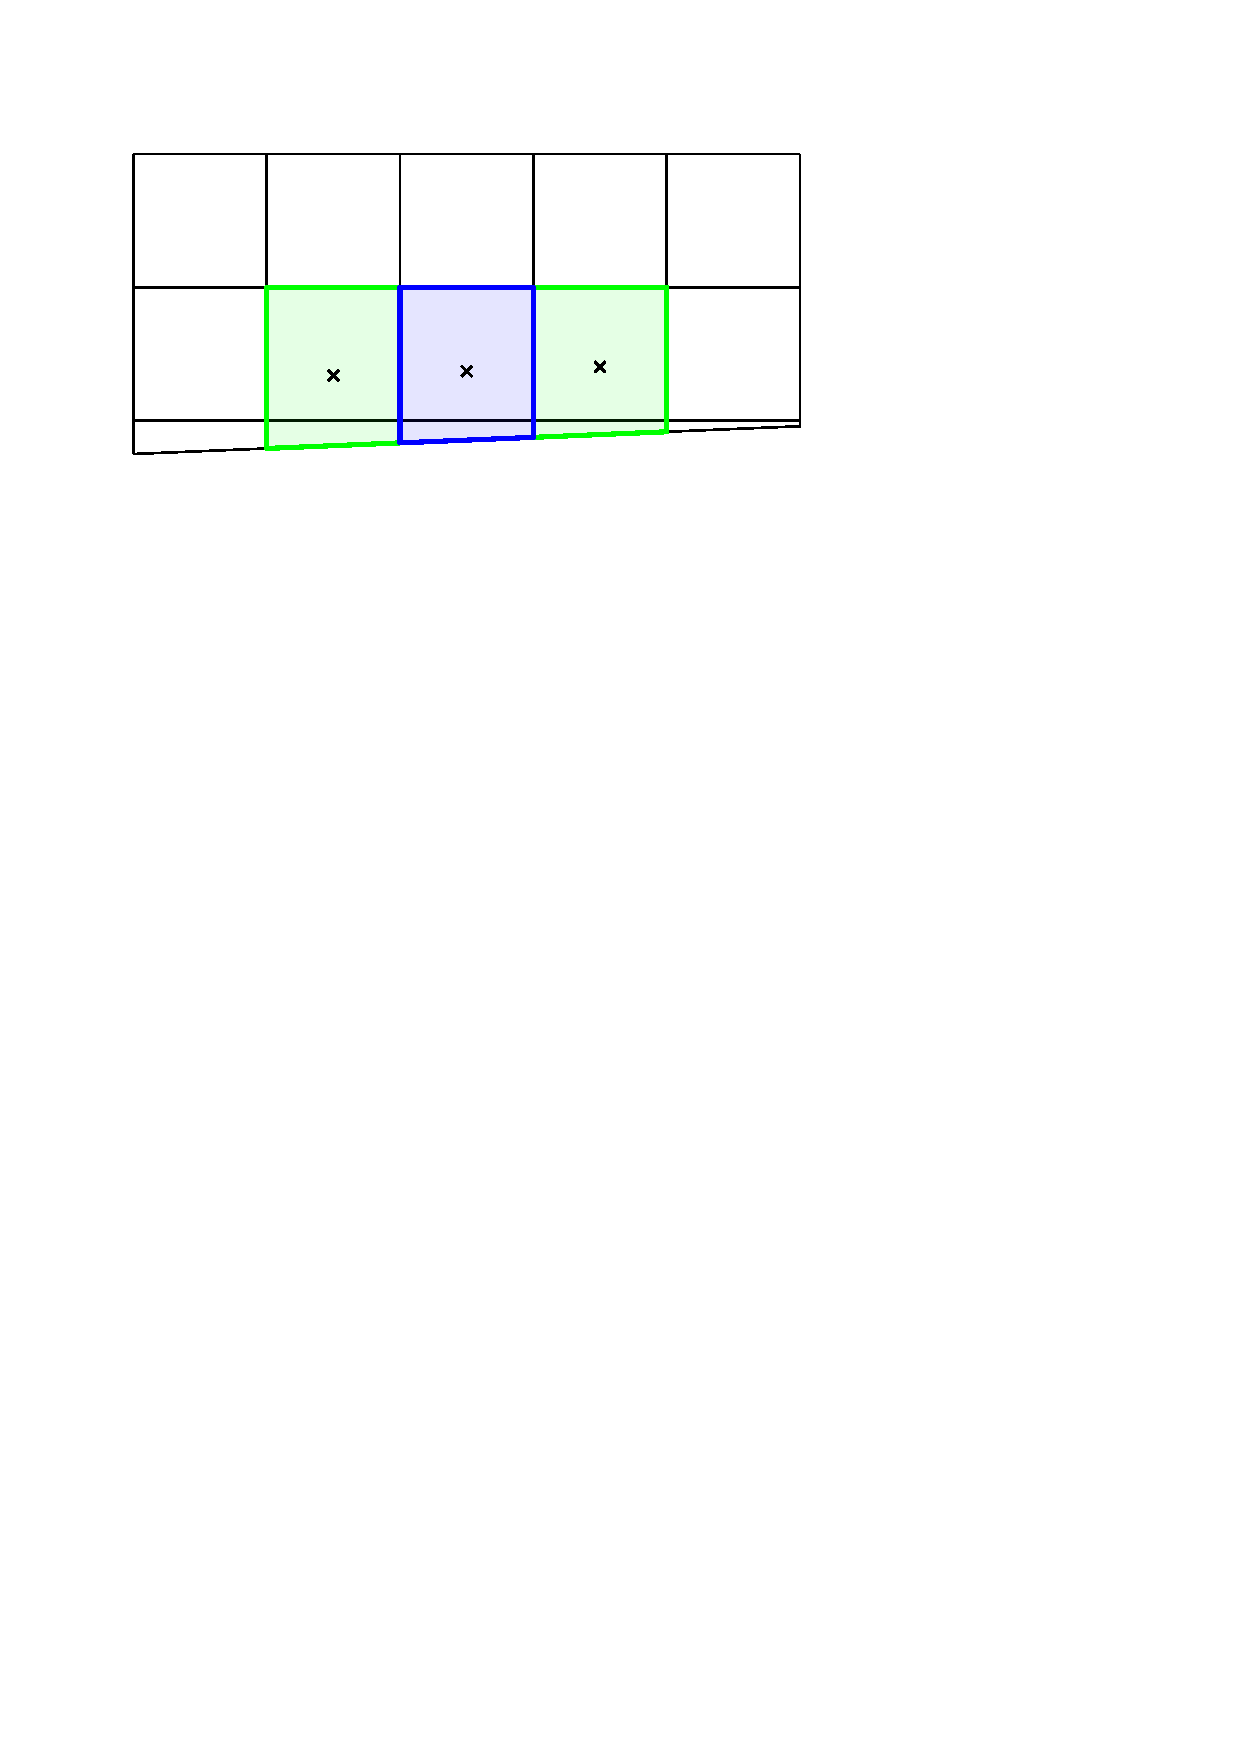
\includegraphics[width=0.30\linewidth]{figs/tooclose2.pdf} \label{fig:a}} \hfill
    \subfloat[The green merging neighborhoods are associated with the whole cells $(i-1,j+1)$, $(i,j+1)$, and $(i+1,j+1)$.]{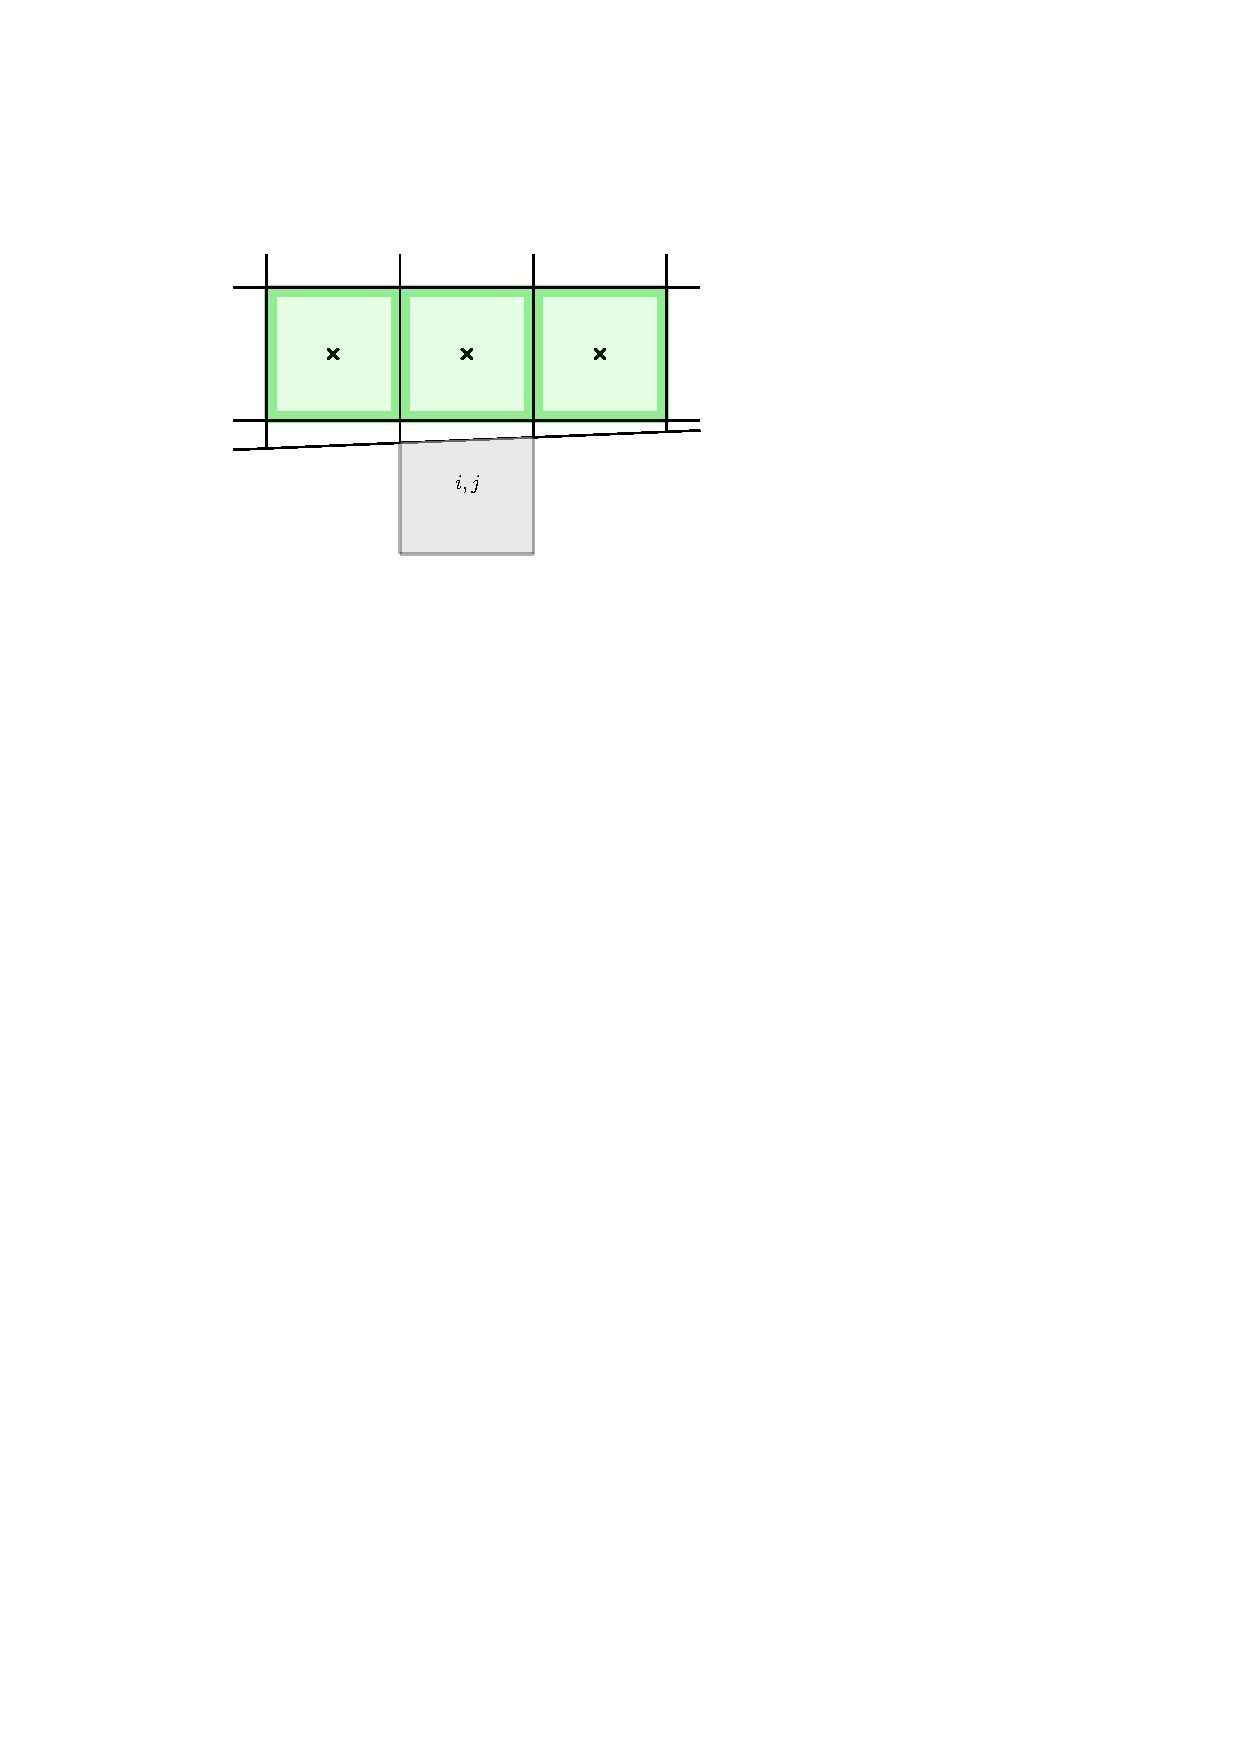
\includegraphics[width=0.30\linewidth]{figs/tooclose1.pdf} \label{fig:b}} \hfill
    \subfloat[The weighted centroids of the reconstruction neighborhoods in Figures \ref{fig:a}, \ref{fig:b}.]{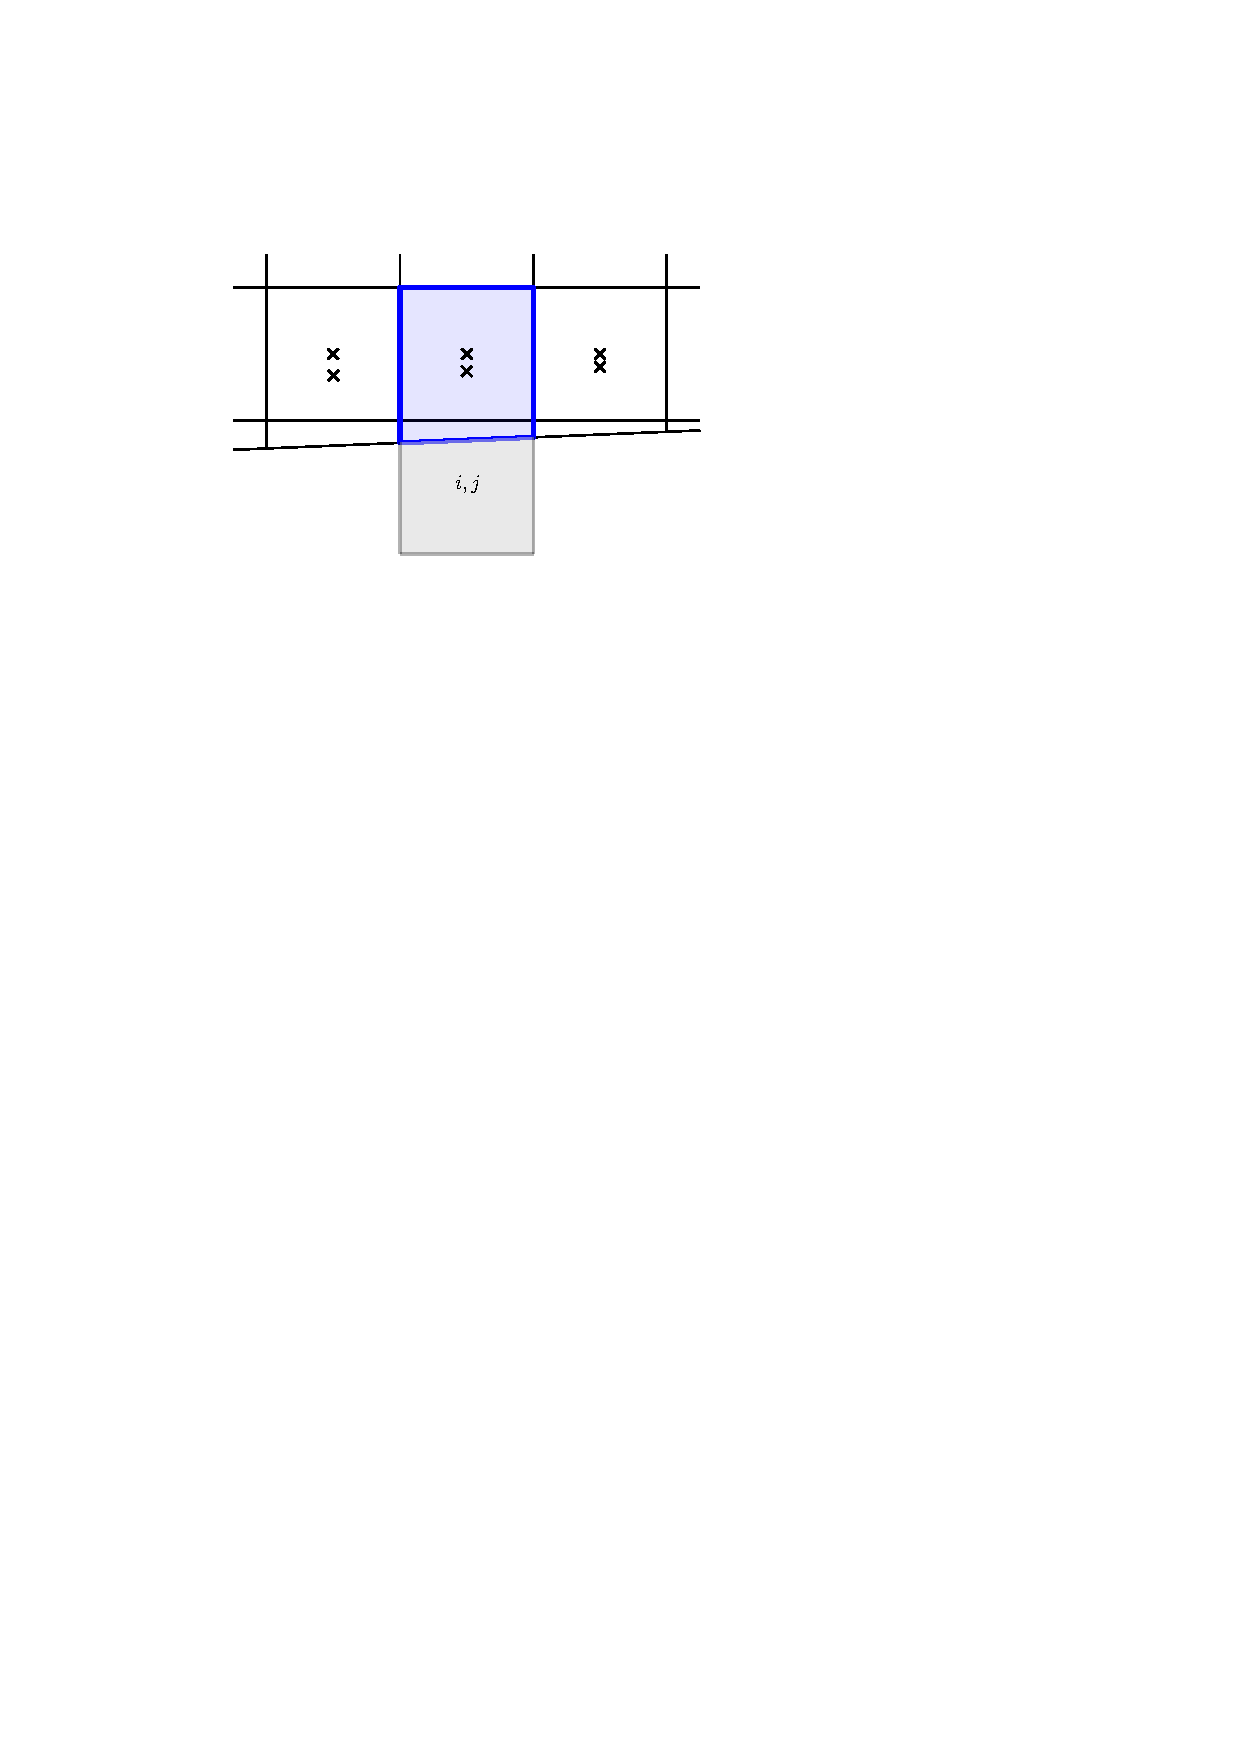
\includegraphics[width=0.30\linewidth]{figs/tooclose3.pdf} \label{fig:c}} 
    \caption{\sf 
%    	In (a) and (b), the blue merging neighborhood's $3\times3$ gradient reconstruction 
%    stencil is highlighted in green.
%    On the right, cell $(i,j+1)$ has a stencil highlighted in green, for computing the gradient in $x$. 
    The weighted centroids of the neighborhoods in $\widehat{R}_{i,j}$ are indicated with a cross ($\times$).  
    Here $\widehat{R}_{i,j}$ is the set of merging neighborhoods associated
    with cells on the $3\times3$ tile centered on cell $(i,j)$.
    Clearly, the weighted centroids are too close to one another in the $y$ direction (Figure \ref{fig:c}).  It follows that least squares system to reconstruct the $x$ and $y$ derivatives of the numerical solution on the blue merging neighborhood is very ill-conditioned.
}
    \label{fig:tooclose}
\end{figure}

%Note that full cells, where the merged  solutions $\widehat{Q}_{i,j} =
%\widehat{U}_{i,j}$ (the
%provisionally updated solution), do not need a gradient. The solution will only be
%evaluated at the cell centroid, which is the same as the neighborhood centroid. 
%Note that the merging neighborhood of the cut cell will
%also contributed to the full cell.

To limit the reconstructed gradient we apply the BJ limiter, this time over $\widehat{R}_{i,j}$
rather than $R_{i,j}$ in \eqref{eqn:bj1} and \eqref{eqn:alpha}.  This procedure is also 
linearity preserving. 
%the points to which the neighborhood solutions are reconstructed in \eqref{eq:bj_alpha}, i.e. $(\widehat{x}_{r,s}, \widehat{y}_{r,s})$, are contained in the convex hull of the points at which the minimum and maximums in \eqref{eqn:bj} are computed \cite{giuliani2018analysis}.


\subsubsection*{Step 3. Final solution update} 

The final update on cell $(i,j)$ is the average of all its neighborhood reconstructions 
evaluated at $(i,j)$'s physical centroid $(x_{i,j},y_{i,j})$. 
This is given by 
\begin{equation} \label{eqn:final_update_linear}
U^{n+1}_{i,j} =   \frac{1}{N_{i,j}}\sum_{(r,s)  \in W_{i,j}}\hat{q}_{r,s}(x_{i,j},y_{i,j}).
\end{equation}
where $W_{i,j}$ is the list of indices of the neighborhoods that overlap cell $(i,j)$.

\vspace*{.5in}

%\noindent\textit{Note 1}: when we are stabilizing the method of lines scheme, $U^{n+1}_{i,j}$ corresponds to either the first or second stage of Heun's method, i.e., $U^{(1)}_{i,j}$ or $U^{(2)}_{i,j}$ in \eqref{eq:molscheme}.  
%Thus, the method of lines scheme in \eqref{eq:molscheme} when stabilized by state redistribution becomes
%\begin{equation}\label{eq:molscheme_srd}
%\begin{aligned}
%\mathbf{U}^{(1)} &= S(\mathbf{U}^{n} + \Delta t L(\mathbf{U}^n)), \\
%\mathbf{U}^{(2)} &= S(\mathbf{U}^{(1)} + \Delta t L(\mathbf{U}^{(1)})), \\
%\mathbf{U}^{n+1} &= \frac{1}{2}( \mathbf{U}^{n} + \mathbf{U}^{(2)} ) ,	
%\end{aligned}
%\end{equation}
%where $S$ is the linear state redistribution operator applied after each forward Euler step of Heun's method.
%When we are stabilizing the MUSCL scheme $U^{n+1}_{i,j}$ has the same meaning as in \eqref{eq:musclscheme}.  Thus, the MUSCL scheme in \eqref{eq:musclscheme} when stabilized by state redistribution becomes
%\begin{equation}\label{eq:musclscheme_srd}
%\mathbf{U}^{n+1} = S(\mathbf{U}^{n} + \Delta t L(\mathbf{U}^{n})).
%\end{equation}

\noindent\textit{Note }: The final update formula \eqref{eqn:final_update_linear} can easily be implemented with a 
nested for loop as in Algorithm \ref{alg:finalupdate},  
instead of computing the set $W_{i,j}$ in \eqref{eqn:final_update_linear}.  
The outer loop iterates over the merging neighborhoods $(i,j)$ and the inner loop iterates over each cell $(r,s)$ in neighborhood $(i,j)$.  Each merging neighborhood $(i,j)$ gives a contribution $ \hat{q}_{i,j}(x_{r,s}, y_{r,s})/N_{r,s} $ to the cells $(r,s)$ that belong to it. 
\begin{algorithm}[H]
		\caption{\sf Final solution update} \label{alg:finalupdate}
	\begin{algorithmic}
	\For{$i,j$}
	\State $U^{n+1}_{i,j} \leftarrow 0$
	\EndFor
	\For{$i,j$}
		\For{$(r,s) \in M_{i,j}$}
			\State $U^{n+1}_{r,s} \leftarrow U^{n+1}_{r,s} + \hat{q}_{i,j}(x_{r,s}, y_{r,s})/N_{r,s} $
		\EndFor
	\EndFor
	\end{algorithmic}
\end{algorithm}


%To use the example of figure \ref{fig:2nborTile}, the cut cell value
%\begin{equation}
%   U_{i,j}^{n+1} := \widehat{Q}_{i,j} 
%   + ( x_{i,j} - \widehat x_{i,j}) \, \widehat{\sigma}_{x,i,j}
%   + ( y_{i,j} - \widehat y_{i,j}) \, \widehat{\sigma}_{y,i,j}
%\end{equation}
%since cell $(i,j)$ only belongs to one neighborhood. The adjacent full cell
%$(i,j+1)$ on the other hand belongs to two neighborhoods -- the one it 
%shares with
%the cut cell $(i,j)$ , and its own merging neighborhood.
%So its solution at time $t^{n+1}$  becomes
%\begin{equation}
%\label{eqn:numhood2ex}
%\begin{split}
%   U_{i,j+1}^{n+1} \,=\, & \frac{1}{2} \, \widehat{q}_{i,j}(x_{i,j+1},y_{i,j+1})+ 
%   \frac{1}{2} \,  \widehat{q}_{i,j+1}(x_{i,j+1},y_{i,j+1}), \\
%   = &\frac{1}{2} \left
%   (\widehat{Q}_{i,j} 
%   + ( x_{i,j+1} - \widehat x_{i,j}) \, \widehat{\sigma}_{x,i,j}
%   + ( y_{i,j+1} - \widehat y_{i,j}) \, \widehat{\sigma}_{y,i,j} \right ) + 
%   \frac{1}{2} \, \widehat{Q}_{i,j+1} .
%\end{split}
%\end{equation}
%The last term  in eq. \eqref{eqn:numhood2ex} has no gradient terms because the
%centroids of the original cell and merged cell are identical.
%The fraction $\frac{1}{2}$ is because cell $(i,j+1)$ is part of  two
%neighborhoods, so each contributes half of the solution.


%One might at first think that only the cut cell need to have its solution replaced
%by the more stable update.  This would not be conservative however; the adjacent cell
%also needs to be part of the update. In addition, each of these cells might also be part of
%another neighborhood if the geometry curves, for example. So in the general case,
%each contribution from a merging tile has to be weighted by the number of
%neigborhoods it contributes to. 






%The conservation properties of the algorithm will be discussed after the
%higher order SRD algorithm is presented in the next
%section. It will also be presented more generally.   

%Different choices of neighborhoods, the minimum volume for the merging
%neighborhood, gradient neighborhoods, and limiting will give
%somewhat different computational results. 
%Some of these will be examined
%theoretically using model problems in one space dimension in section
%\ref{sec:theory}. These choices can affect the stability limit of the
%overall method.
%We will also show computational results using different neighborhood
%choices in section \ref{sec:compResults} in two space dimensions.

\subsection{Linear exactness} \label{sec:linex}
In this section, we show that second order accurate state redistribution preserves linear functions.
One might wonder about this since the centroids and solution averages are weighted in this unusual way.
In addition, the local truncation error does not imply the order of
accuracy of the scheme  as it does on regular meshes \cite{Kreiss:white2}. 
Here we simply show that a
linear function remains exact after SRD, if the base scheme is linearly
exact.
%If all cells had the same number of neighborhoods in \eqref{34} the $N_{ij}$ would all cancel. 
%Since they do not, it is harder to have an intuition about this.

Consider the grid function of the numerical solution after one time step
or stage, $\widehat{U}$.  Assume that it can be written in terms of a linear function $f(x,y)$ of the $x$ and $y$ coordinates, i.e.,
\begin{equation}
    \label{eqn:uhatlinear}
\widehat{U}_{i,j} = f(x_{i,j},y_{i,j}) = ax_{i,j} + by_{i,j} + c.
\end{equation}
This assumption is valid since both the method of lines (Section \ref{sec:mol}) and the MUSCL scheme (Section \ref{sec:muscl}) are linearity preserving.  
%That is, after one step or stages of these numerical methods, a linear solution remains linear.
From \eqref{eqn:uhatlinear} and the expression for the average on the merging neighborhood $(i,j)$ in \eqref{tiledef}, we have
\begin{equation}
    \label{eqn:linear1}
\widehat{Q}_{i,j} = \frac{1}{{\widehat V}_{i,j}} \, \sum_{(r,s) \in M_i} \,  
\frac{V_{r,s}}{N_{r,s}}  \,\, (ax_{r,s} + by_{r,s} + c).
\end{equation}
Distributing the summation in \eqref{eqn:linear1}, we have
\begin{equation}\label{eqn:linear2}
\widehat{Q}_{i,j} =  a \left(\frac{1}{{\widehat V}_{i,j}} \, \sum_{(r,s) \in M_{i,j}} \,  
\frac{V_{r,s}}{N_{r,s}} x_{r,s} \right) + b\left(\frac{1}{{\widehat V}_{i,j}} \, \sum_{(r,s) \in M_{i,j}} \,  
\frac{V_{r,s}}{N_{r,s}} y_{r,s} \right) + c\left(\frac{1}{{\widehat V}_{i,j}} \, \sum_{(r,s) \in M_{i,j}} \,
\frac{V_{r,s}}{N_{r,s}}\right) .
\end{equation}
From the definition of the weighted centroid and volume of the merging neighborhood
$(i,j)$ in \eqref{eqn:voldef} and \eqref{eqn:centroiddef}, respectively, \eqref{eqn:linear2} becomes
\begin{equation}\label{eqn:linear3}
\widehat{Q}_{i,j} =  a \widehat{x}_{i,j} + b\widehat{y}_{i,j} + c = f(\widehat{x}_{i,j},\widehat{y}_{i,j}).
\end{equation}
Now, on neighborhood $(i,j)$, we solve the least squares system 
\eqref{eqn:linrecon} to find $\widehat{\sigma}_{x,i,j}$ and
$\widehat{\sigma}_{y,i,j}$, the gradient on the merging neighborhood.  Using
\eqref{eqn:linear3} in \eqref{eqn:linrecon}, and due to the linearity of $f$, the following system
\begin{equation}
\widehat{\sigma}_{x,i,j}(\widehat{x}_{r,s} - \widehat{x}_{i,j}) + \widehat{\sigma}_{y,i,j}(\widehat{y}_{r,s} - \widehat{y}_{i,j})= f(\widehat{x}_{r,s}, \widehat{y}_{r,s}) - f(\widehat{x}_{i,j}, \widehat{y}_{i,j}) \quad \forall (r,s) \in \widehat{R}_{i,j},
\end{equation}
is solved exactly by $\widehat{\sigma}_{x,i,j}=a$ and
$\widehat{\sigma}_{y,i,j}=b$.  In other words, the exact gradient 
of $f$ is reconstructed on merging neighborhood $(i,j)$.  
The reconstructed solution is then
\begin{equation}
    \label{eqn:qrecon1}
    \hat{q}_{i,j}(x,y) = f(\widehat{x}_{i,j},\widehat{y}_{i,j}) + a(x-\widehat{x}_{i,j})+b(y-\widehat{y}_{i,j}) .
\end{equation}
Using \eqref{eqn:linear3}, \eqref{eqn:qrecon1} becomes
\begin{equation}
    \label{eqn:qrecon2}
    \hat{q}_{i,j}(x,y) = f(x,y).
\end{equation}
By \eqref{eqn:final_update_linear}, the final solution update is
\begin{equation} 
U^{n+1}_{i,j} = \frac{1}{N_{i,j}}\sum_{(r,s) \in W_{i,j}}f(x_{i,j},y_{i,j}).
\end{equation}
The function values are exact, and there are $N_{i,j}$ of them, so
after dividing by $N_{i,j}$ we get
\begin{equation} 
U^{n+1}_{i,j} = f(x_{i,j},y_{i,j}),
\end{equation}
which shows that second order accurate state redistribution preserves linear functions.
%Numerical experiments in Section \ref{sec:compResults} will demonstrate the scheme's order of accuracy.



\subsection{Conservation}\label{sec:cons}
In this section, we show that the total mass of the numerical solution before and after state redistribution does not change.  It follows from the final update in \eqref{eqn:final_update_linear} that the total mass after state redistribution is
\begin{equation}\label{eq:mi}
\sum_{i,j} V_{i,j} U^{n+1}_{i,j} = \sum_{i,j} \sum_{(r,s) \in
M_{i,j}}\frac{1}{N_{r,s}} V_{r,s} \widehat q_{i,j}(x_{r,s},y_{r,s}) ,
\end{equation}
where $\widehat q_{i,j}(x)$ is that neighborhood's polynomial reconstruction defined in \eqref{eq:qrecon}.
Using the definition
of $\widehat{q}_{i,j}(x,y)$, we have
\begin{equation}\label{eq:mi1}
\sum_{i,j} V_{i,j} U^{n+1}_{i,j} = \sum_{i,j} \widehat {Q}_{i,j} 
\widehat {V}_{i,j}.
\end{equation}
Using the definition of the weighted average \eqref{tiledef}, we have
\begin{equation}\label{eq:mi2}
\sum_{i,j} V_{i,j} U^{n+1}_{i,j} = \sum_{i,j} \sum_{(r,s) \in M_{i,j} }\frac{V_{r,s}}{N_{r,s}} \widehat U_{r,s}.
\end{equation}
Since $N_{r,s}$ indicates the number of times cell $(r,s)$ is overlapped by merging neighborhoods, it follows that the $\frac{V_{r,s}}{N_{r,s}} \widehat U_{r,s}$ term is repeated $N_{r,s}$ times in the sum of \eqref{eq:mi2}.  Thus, simplifying \eqref{eq:mi2}, it follows that
\begin{equation} \label{eq:final}
\sum_{i,j} V_{i,j} U^{n+1}_{i,j} = \sum_{i,j} V_{i,j} \widehat U_{i,j}
\end{equation}
and the total mass before and after state redistribution is the same.
